\documentclass[a4,landscpae]{seminar}
\pdfcompresslevel=9
\pdfpagewidth=11.69 truein % A4 portrait
\pdfpageheight=8.27 truein % A4 portrait
\pdfhorigin=1truein     % default value(?), but doesn't work without
\pdfvorigin=1truein     % default value(?), but doesn't work without
\slideheight=17.5cm
\slidewidth=23cm

\usepackage[spanish]{babel}
\usepackage[latin1]{inputenc}

\usepackage{t-gsyc-6}
\usepackage{fancybox}
\usepackage{graphics}
\usepackage{moreverb}
\usepackage{alltt}
\usepackage{amsmath}
\usepackage[normalsize]{subfigure}
\usepackage{url}

\title{HACIENDO PROGRAMABLE Y ESTABLE CON FPGA UN DRONE COMERCIAL}
\author{Eloy Navarro Morales}
\conference{Trabajo Fin de Grado}

\cop{E. Navarro}
\begin{document}
\maketitle

%%--------------------------------------------------------------
%% INDICE
%%--------------------------------------------------------------
\begin{hslide}
\slsect{\'Indice}
\begin{itemize}
	\item Introducci\'on
	\item Objetivos
	\item Infraestructura
	\item Dron comercial programable
	\item Validaci\'on experimental
	\item Conclusiones
\end{itemize}
\end{hslide}



%%--------------------------------------------------------------
%% INTRODUCCION
%%--------------------------------------------------------------
\begin{hslide}
\slsect{Introducci\'on}
\slsubsect{Drones}
\begin{minipage}{6.1cm}
	\begin{figure}
		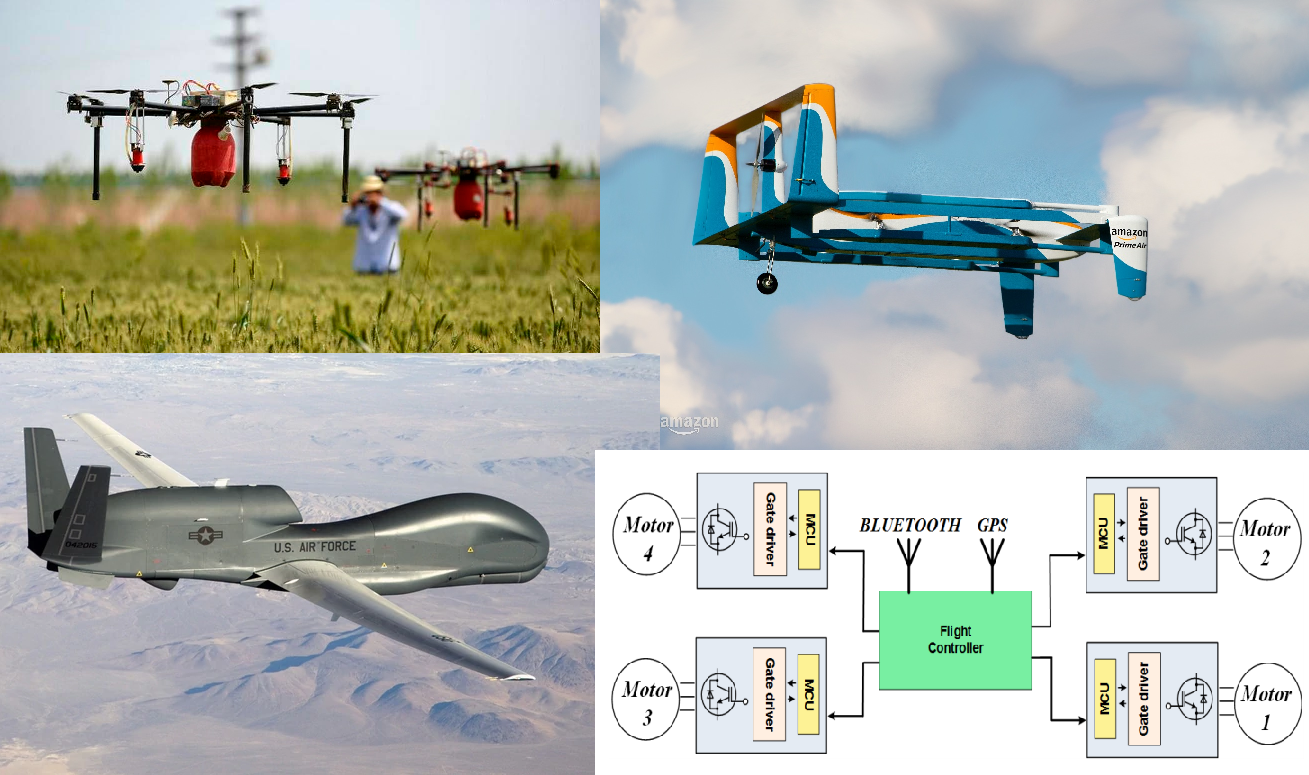
\includegraphics[width=6.2cm]{Imagenes/Intro_Drones}
	\end{figure}
\end{minipage} \hfill
\begin{minipage}{4.9cm}
	\begin{itemize}
		\item Aplicaciones en entorno civil y militar
		\item Sistemas de control variados seg\'un aplicaci\'on
	\end{itemize}
\end{minipage}

\end{hslide}
%%--------------------------------------------------------------
\begin{hslide}
\slsubsect{FPGAs}
\begin{minipage}{7cm}
	\begin{center}
		\begin{figure}
			%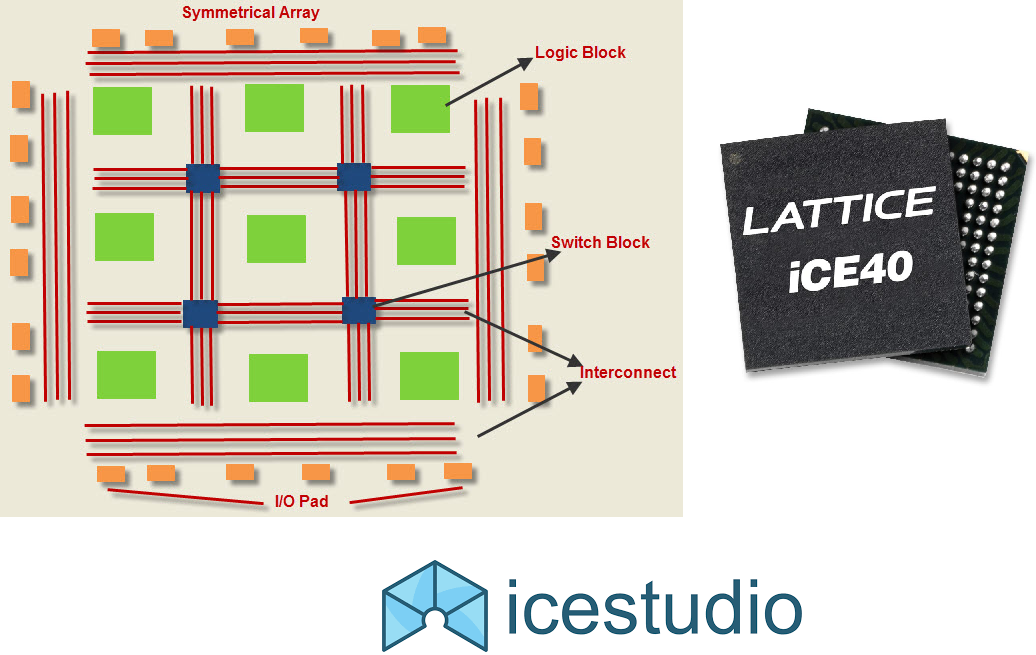
\includegraphics[width=8cm]{Imagenes/Intro_FPGA}
			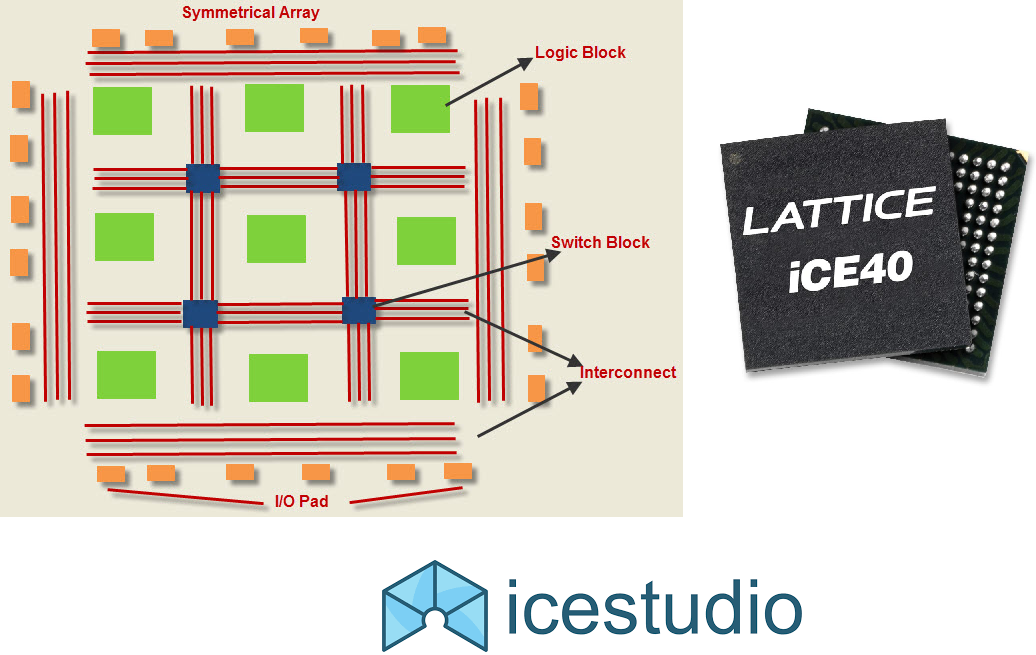
\includegraphics[width=7.5cm]{Imagenes/Intro_FPGA}
		\end{figure}
	\end{center}
\end{minipage} \hfill
\begin{minipage}{3.5cm}
	\begin{itemize}
		\item Potencia paralela
		\item Escalabilidad
		\item Reconfiguraci\'on
		\item Desarrollo abierto
	\end{itemize}
\end{minipage}
\end{hslide}
%%---------------------------------------------------------------



%%--------------------------------------------------------------
%% OBJETIVOS
%%--------------------------------------------------------------
\begin{hslide}
\slsect{Objetivos}
Hacer \textbf{estable y programable} el vuelo de un dron comercial de
bajo coste haciendo uso de FPGAs libres

Sub-objetivos:
	\begin{itemize}
		\item Sensorizar veh\'iculo y enlazarlo con tierra
		\item Dise\~nar estaci\'on de tierra y control en comunicaci\'on con dron y PC
		\item Dise\~nar software para PC de mando en Python
	\end{itemize}
\end{hslide}
%%--------------------------------------------------------------
\begin{hslide}
\slsubsect{Requisitos}
	\begin{itemize}
		\item Control en tres grados de libertad independientes
		\item Manejo en tiempo real
		\item Reprogramaci\'on de par\'ametros de control
		\item Instrucciones de manejo de alto nivel
		\item Este apartado quiz\'as sobra?
	\end{itemize}
\end{hslide}



%%--------------------------------------------------------------
%% INFRAESTRUCTURA
%%--------------------------------------------------------------
\begin{hslide}
\slsect{Infraestructura}
\begin{minipage}{6.5cm}
	\slsubsect{Software}
	\begin{itemize}
		\item IDEs: Quartus, IceCube2, ArduinoIDE
		\item Simulaci\'on: ModelSim
		\item Programaci\'on y depuraci\'on: Diamond, FT\_Prog, Logic
	\end{itemize}
	\slsubsect{Hardware}
	\begin{itemize}
		\item Plataformas: Arduino, ICE40, SYMA X5C
		\item Comunicaciones: NRF24L01
		\item Sensores: Flow breakout board

	\end{itemize}
\end{minipage} \hfill
\begin{minipage}{4cm}
	\begin{figure}
		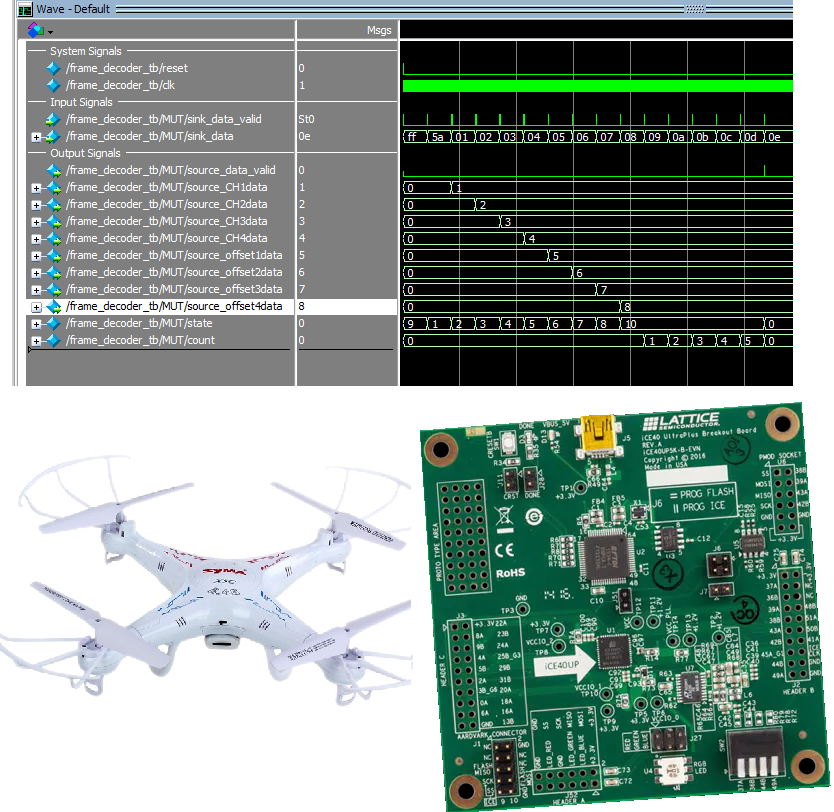
\includegraphics[width=5.2cm]{Imagenes/Infraestructura}
	\end{figure}
\end{minipage} \hfill
\end{hslide}
%%--------------------------------------------------------------



%%--------------------------------------------------------------
%% SISTEMA: DRON COMERCIAL PROGRAMABLE
%%--------------------------------------------------------------
\begin{hslide}
\slsect{Dron comercial programable}
Sistema basado en sensorizaci\'on adicional a bordo del dron e infraestructura de control en tierra\\

\begin{minipage}{4.5cm}
	\slsubsect{M\'odulo en vuelo}
	\begin{itemize}
		\item Dron: Cuadric\'opteros enriquecidos
	\end{itemize}
	\slsubsect{M\'odulos en Tierra}
	\begin{itemize}
		\item PC de mando: Python para el manejo del veh\'iculo
		\item Estaci\'on de tierra basada en FPGA: Verilog para el control
	\end{itemize}
\end{minipage} \hfill
\begin{minipage}{6cm}
	\begin{figure}
		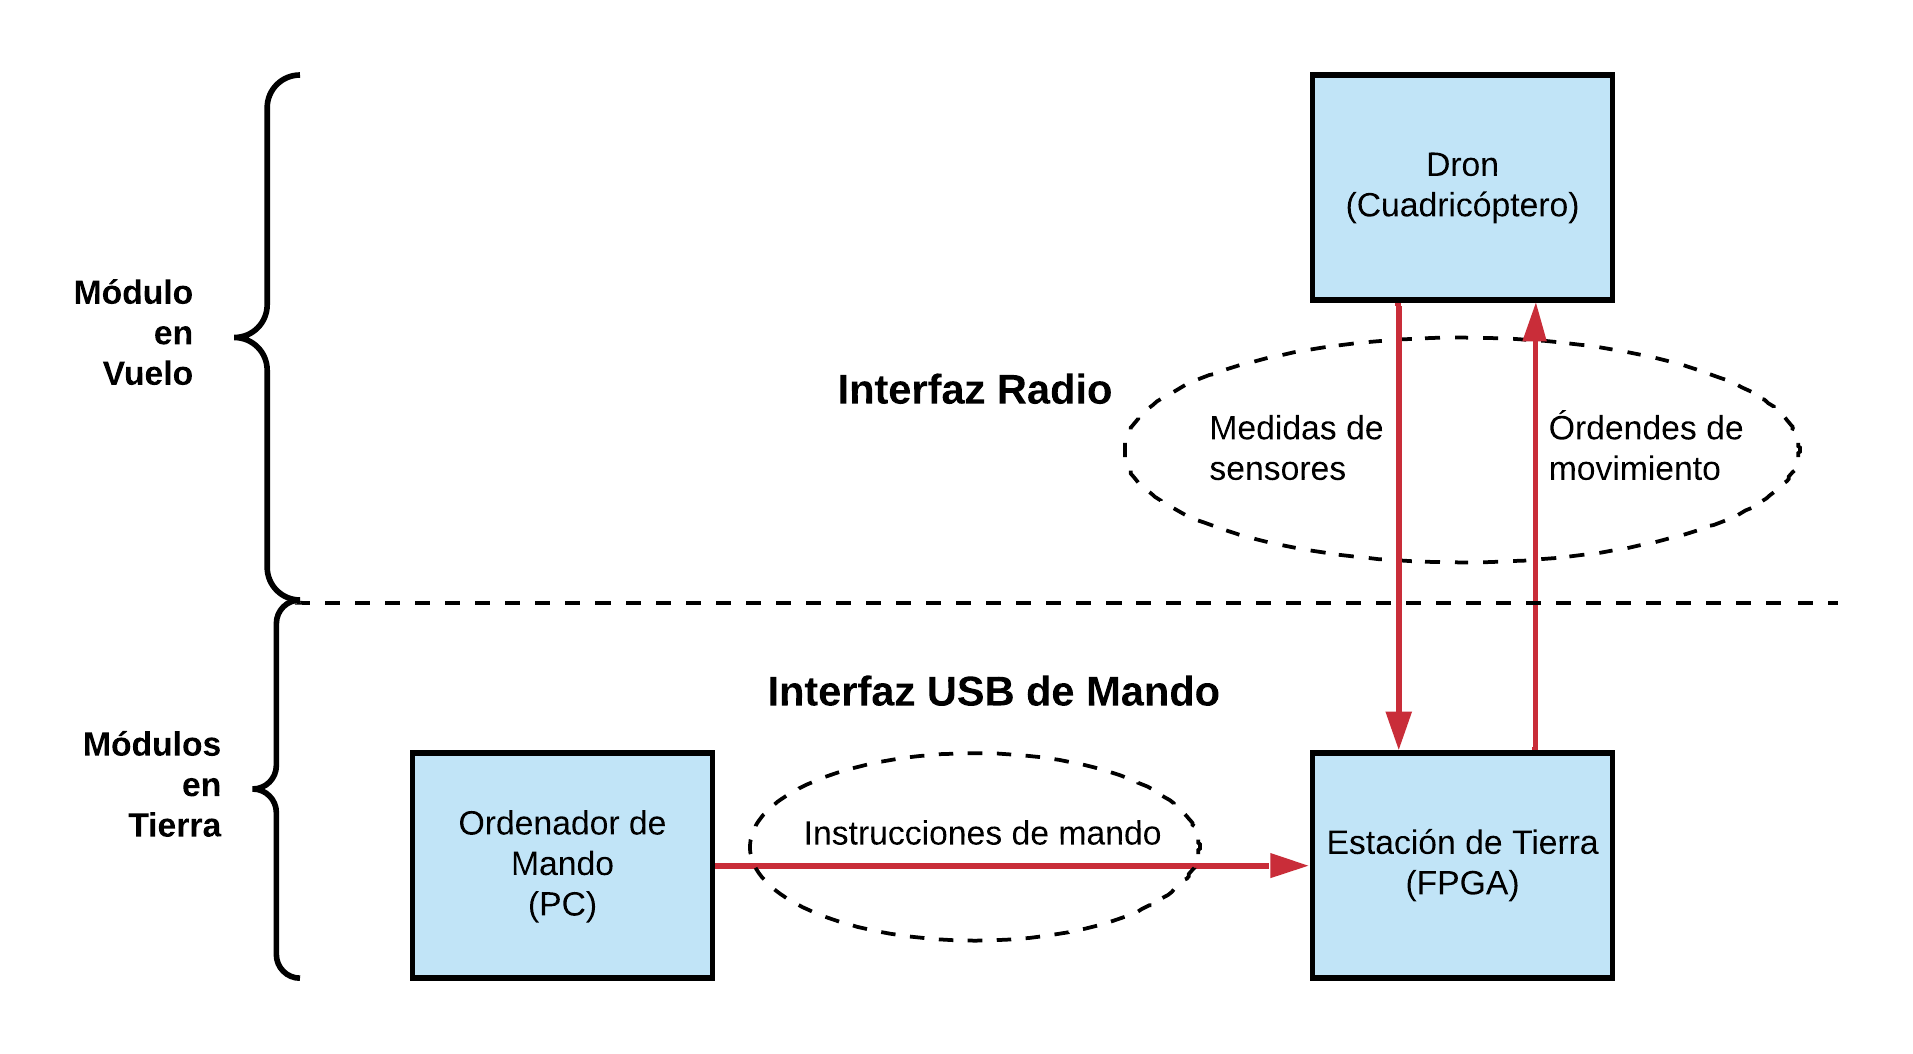
\includegraphics[width=8cm]{Imagenes/Arquitectura_del_Sistema}
	\end{figure}
\end{minipage} \hfill
\end{hslide}
%%--------------------------------------------------------------
\begin{hslide}
\slsubsect{Flujo de control}
\begin{center}
	\begin{figure}[h]
		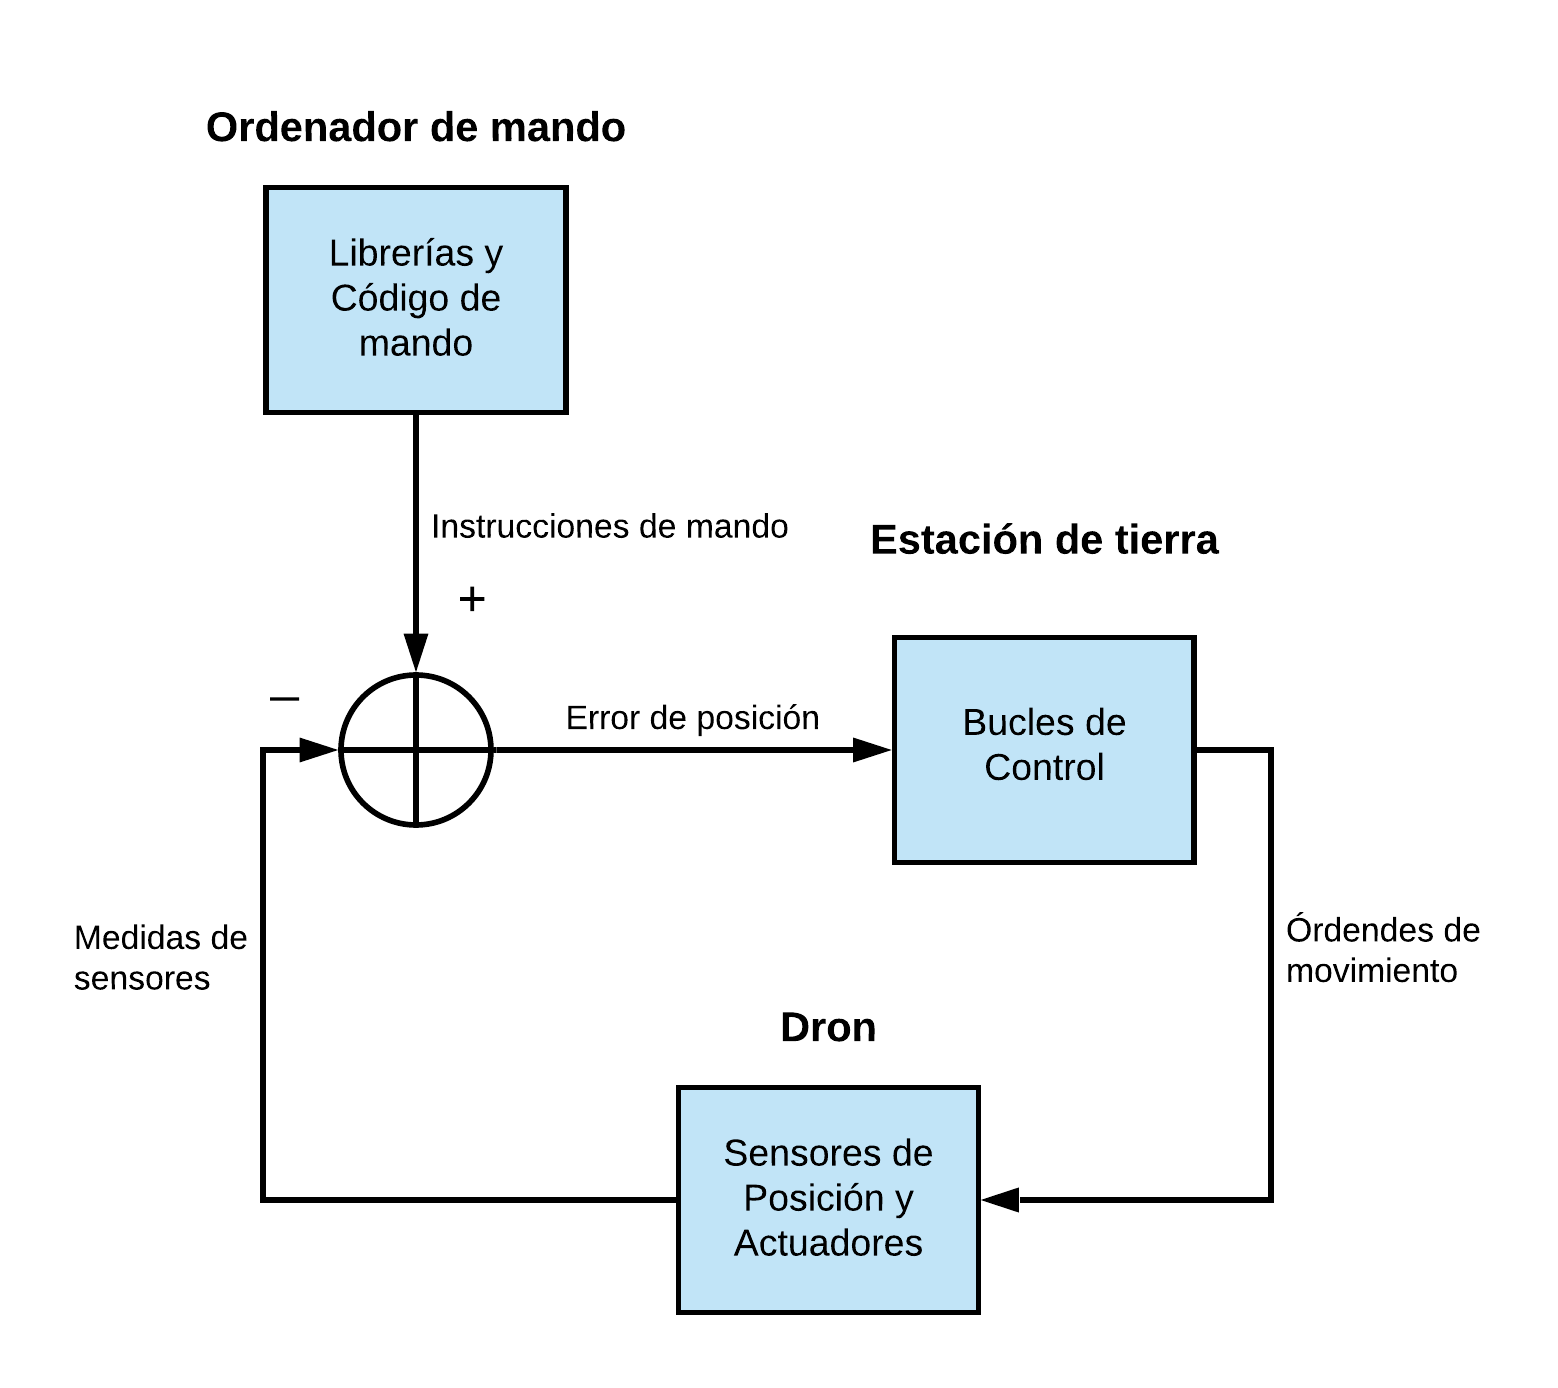
\includegraphics[width=8cm]{Imagenes/Flujo_del_Sistema}
	\end{figure}
\end{center}
\end{hslide}
%%--------------------------------------------------------------
\begin{hslide}
\slsubsect{Dron - Arquitectura}
\begin{minipage}{7cm}
	\begin{center}
		\begin{figure}
			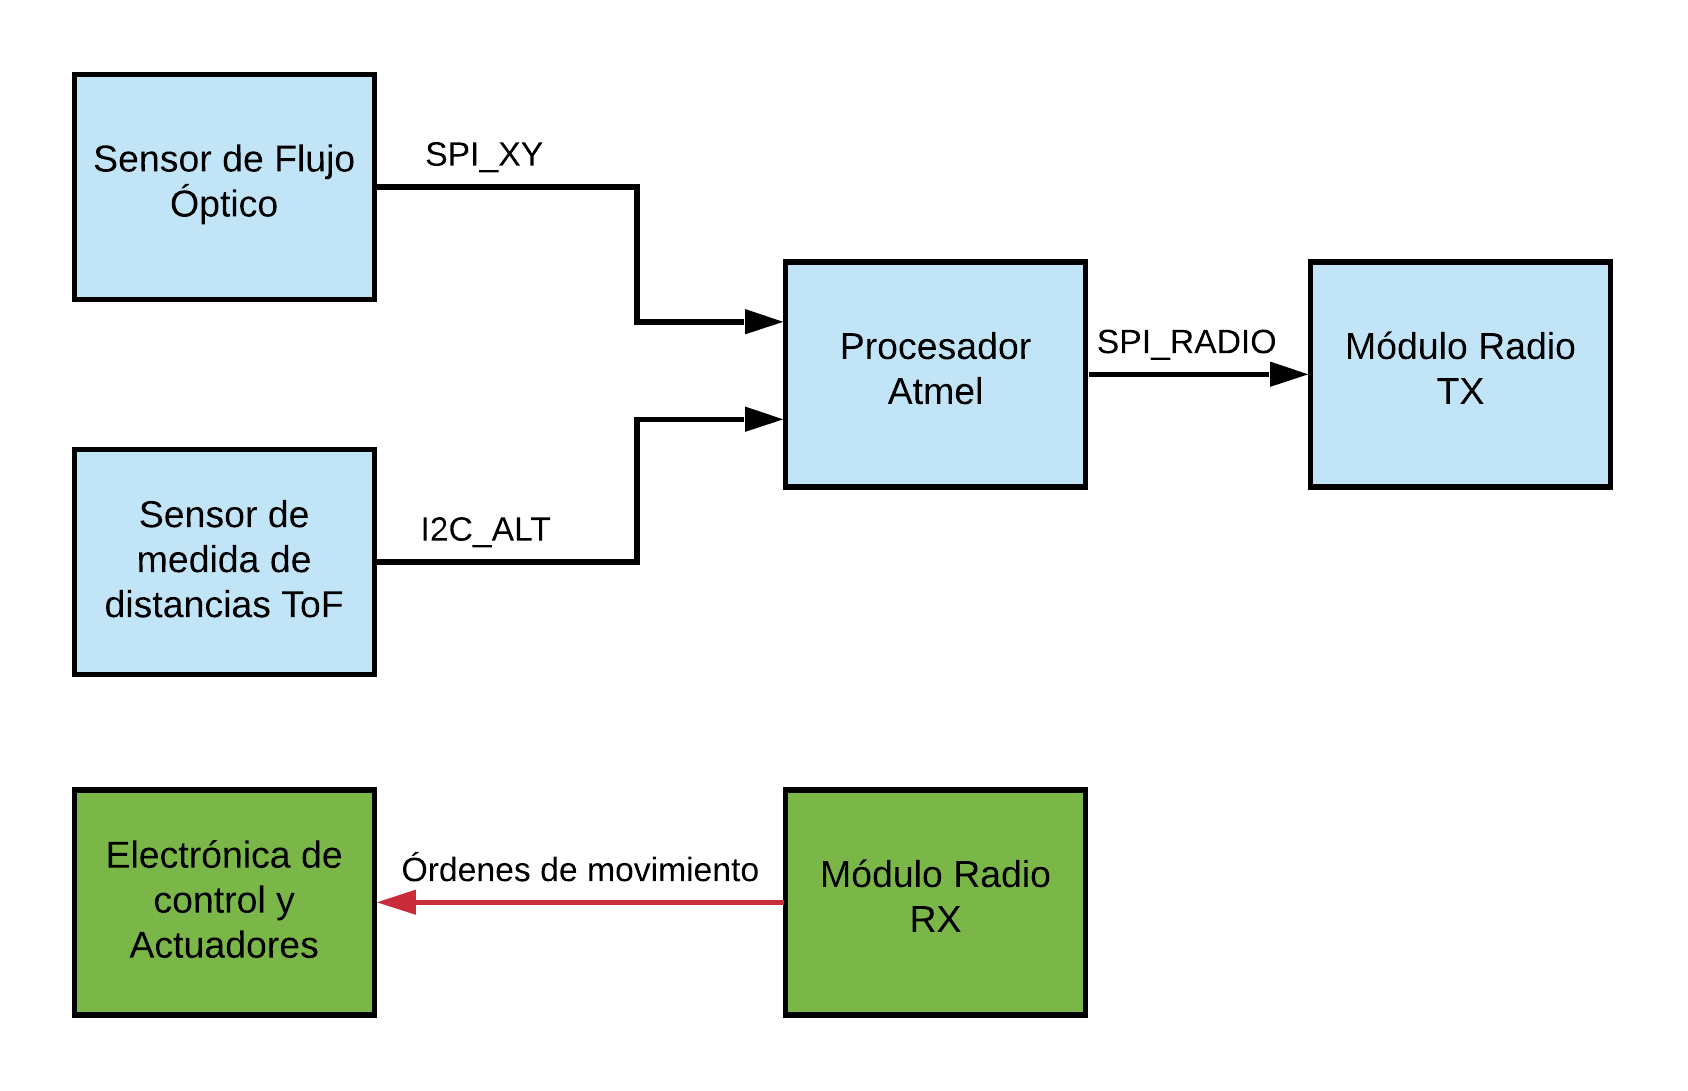
\includegraphics[width=7.5cm]{Imagenes/Drone_arq}
		\end{figure}
	\end{center}
\end{minipage} \hfill
\begin{minipage}{3.9cm}
	\begin{itemize}
		\item Sensoriza:
			\begin{itemize}
				\item Distancia al suelo
				\item Posici\'on horizontal
			\end{itemize}
		\item Transmite medidas
		\item Obedece \'ordenes de movimiento
	\end{itemize}
\end{minipage}
\end{hslide}
%%--------------------------------------------------------------
\begin{hslide}
\slsubsect{Dron - Instalaci\'on}
\begin{minipage}{3cm}
	\begin{center}
		\begin{figure}
			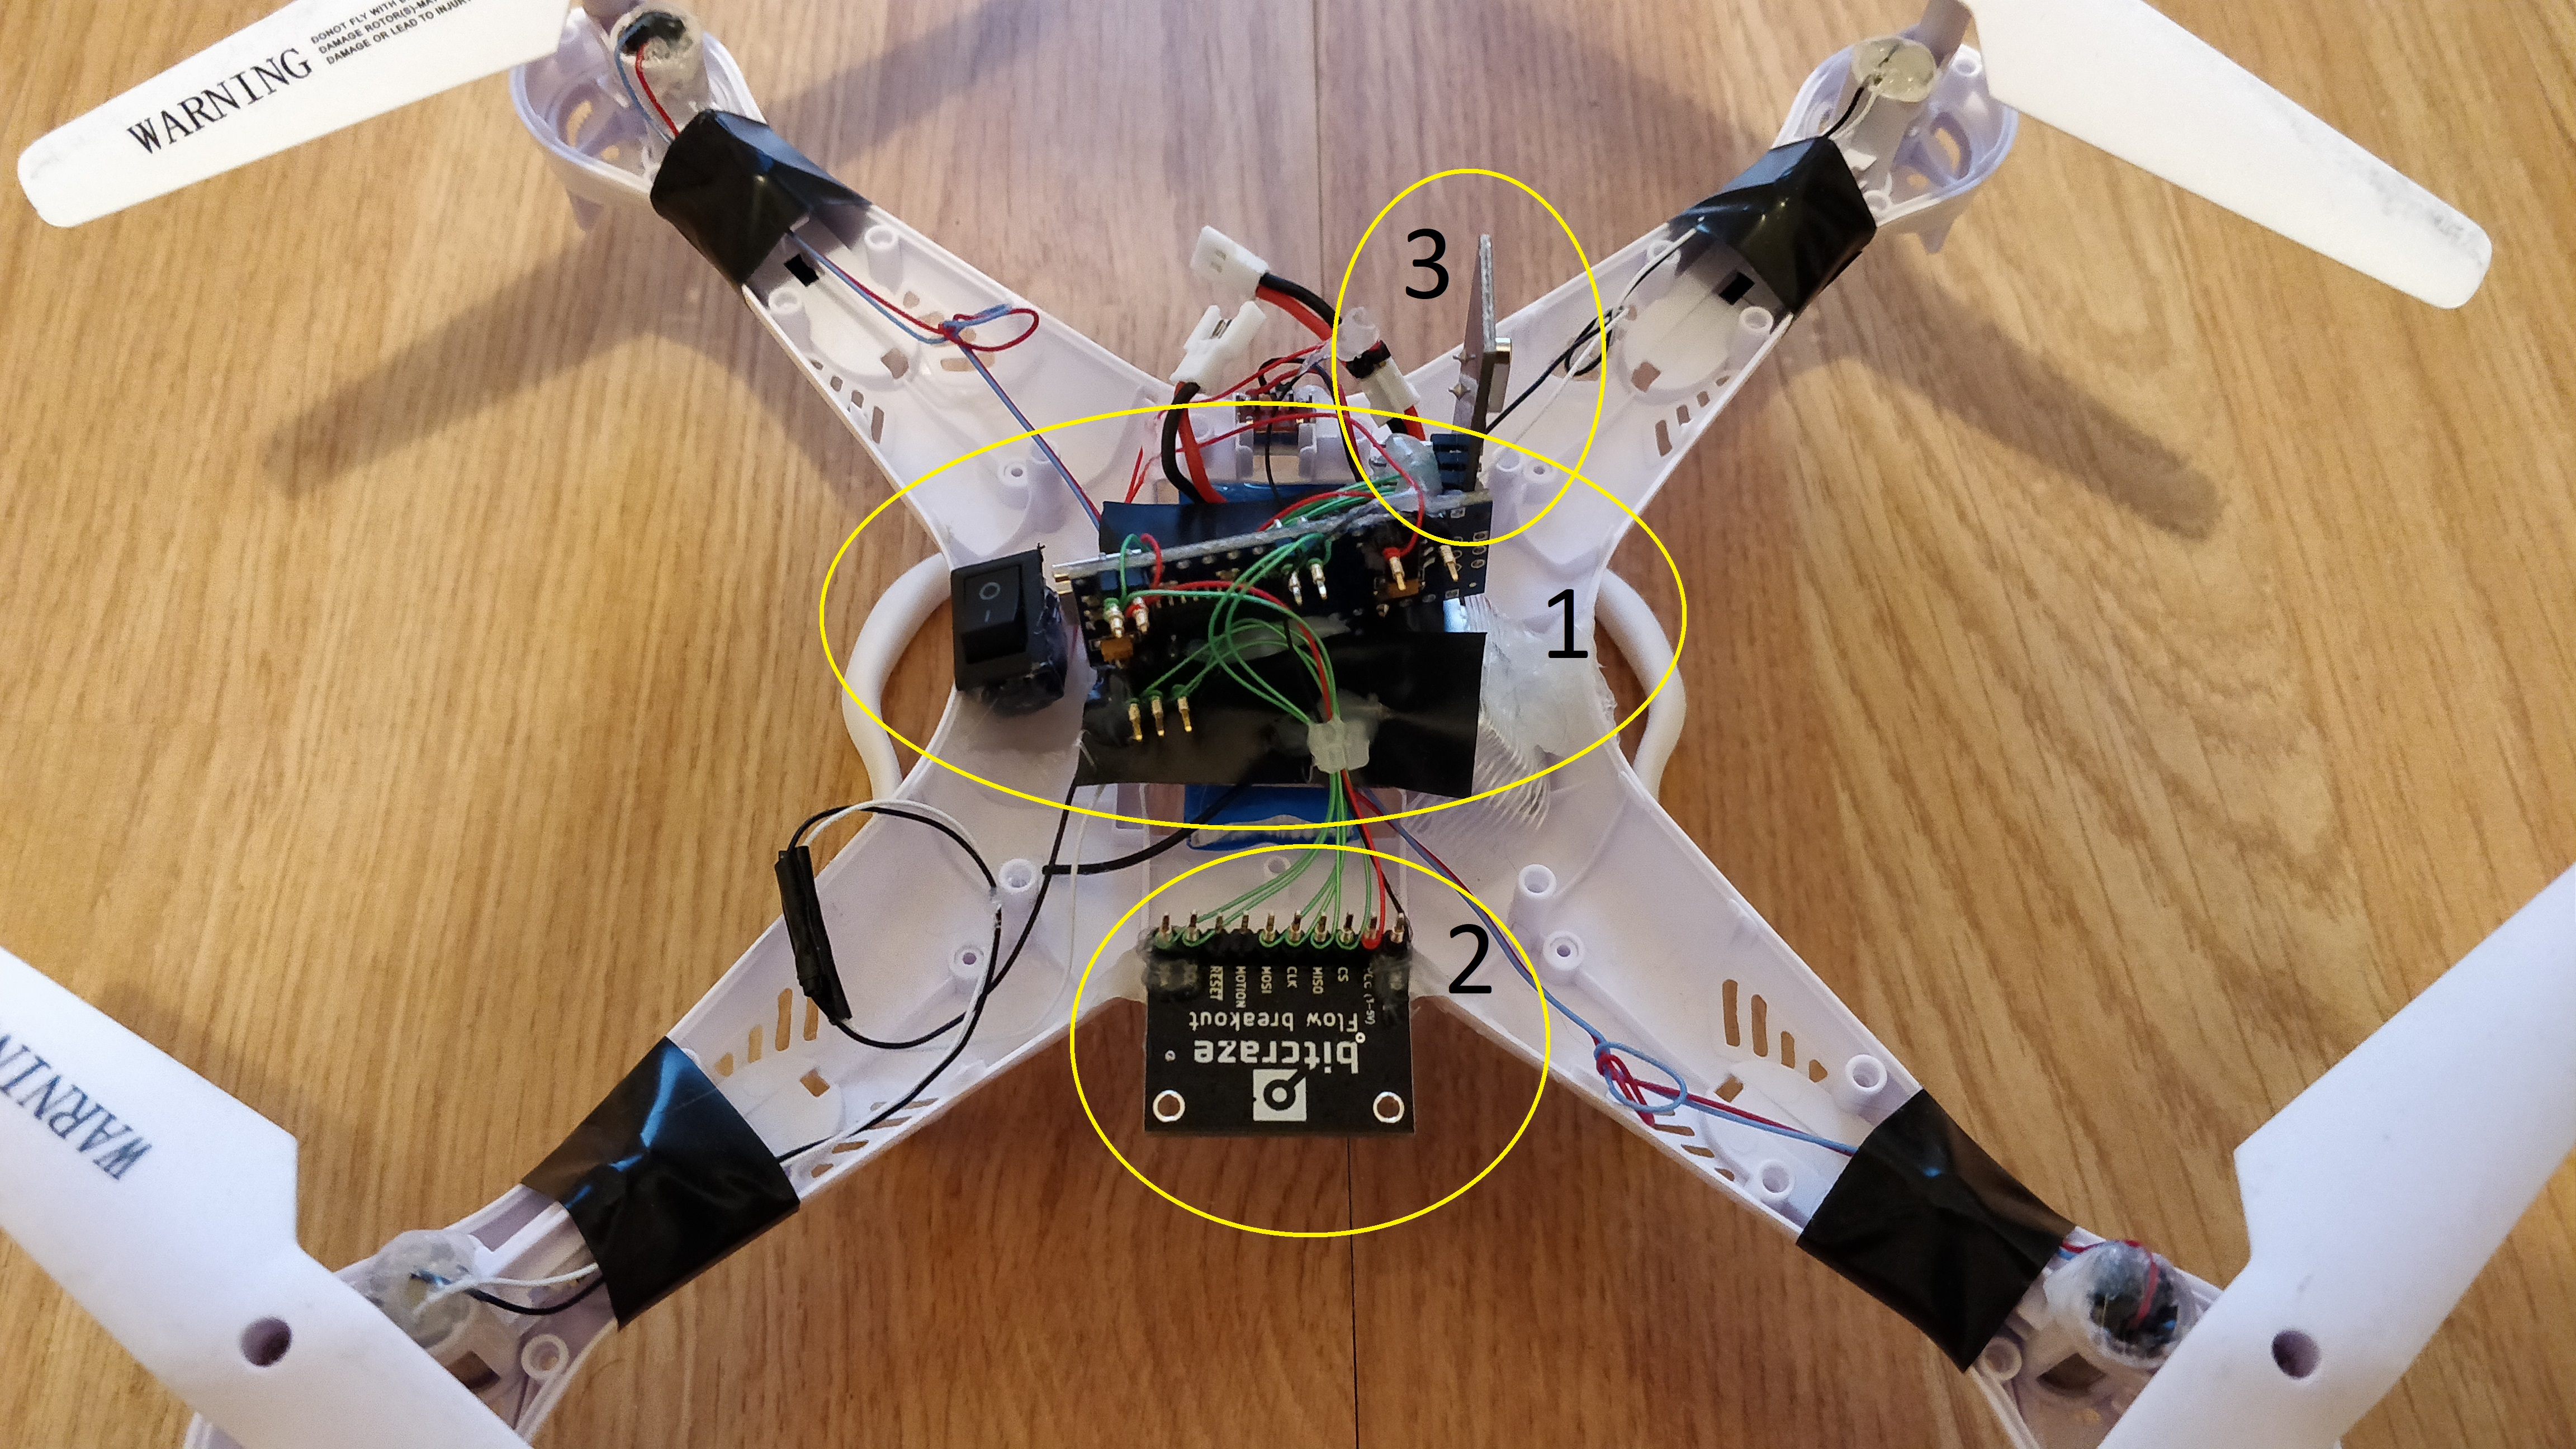
\includegraphics[width=7.8cm]{Imagenes/OnBoard_System_Mod}
		\end{figure}
	\end{center}
\end{minipage} \hfill
\begin{minipage}{2.8cm}
	M\'odulos:
	\begin{itemize}
		\item 1: Procesador
		\item 2: Sensores
		\item 3: Transmisor
	\end{itemize}
\end{minipage}
\end{hslide}
%%--------------------------------------------------------------
\begin{hslide}
\slsubsect{Estaci\'on de tierra basada en FPGA}
\begin{minipage}{3cm}
	\begin{center}
		\begin{figure}
			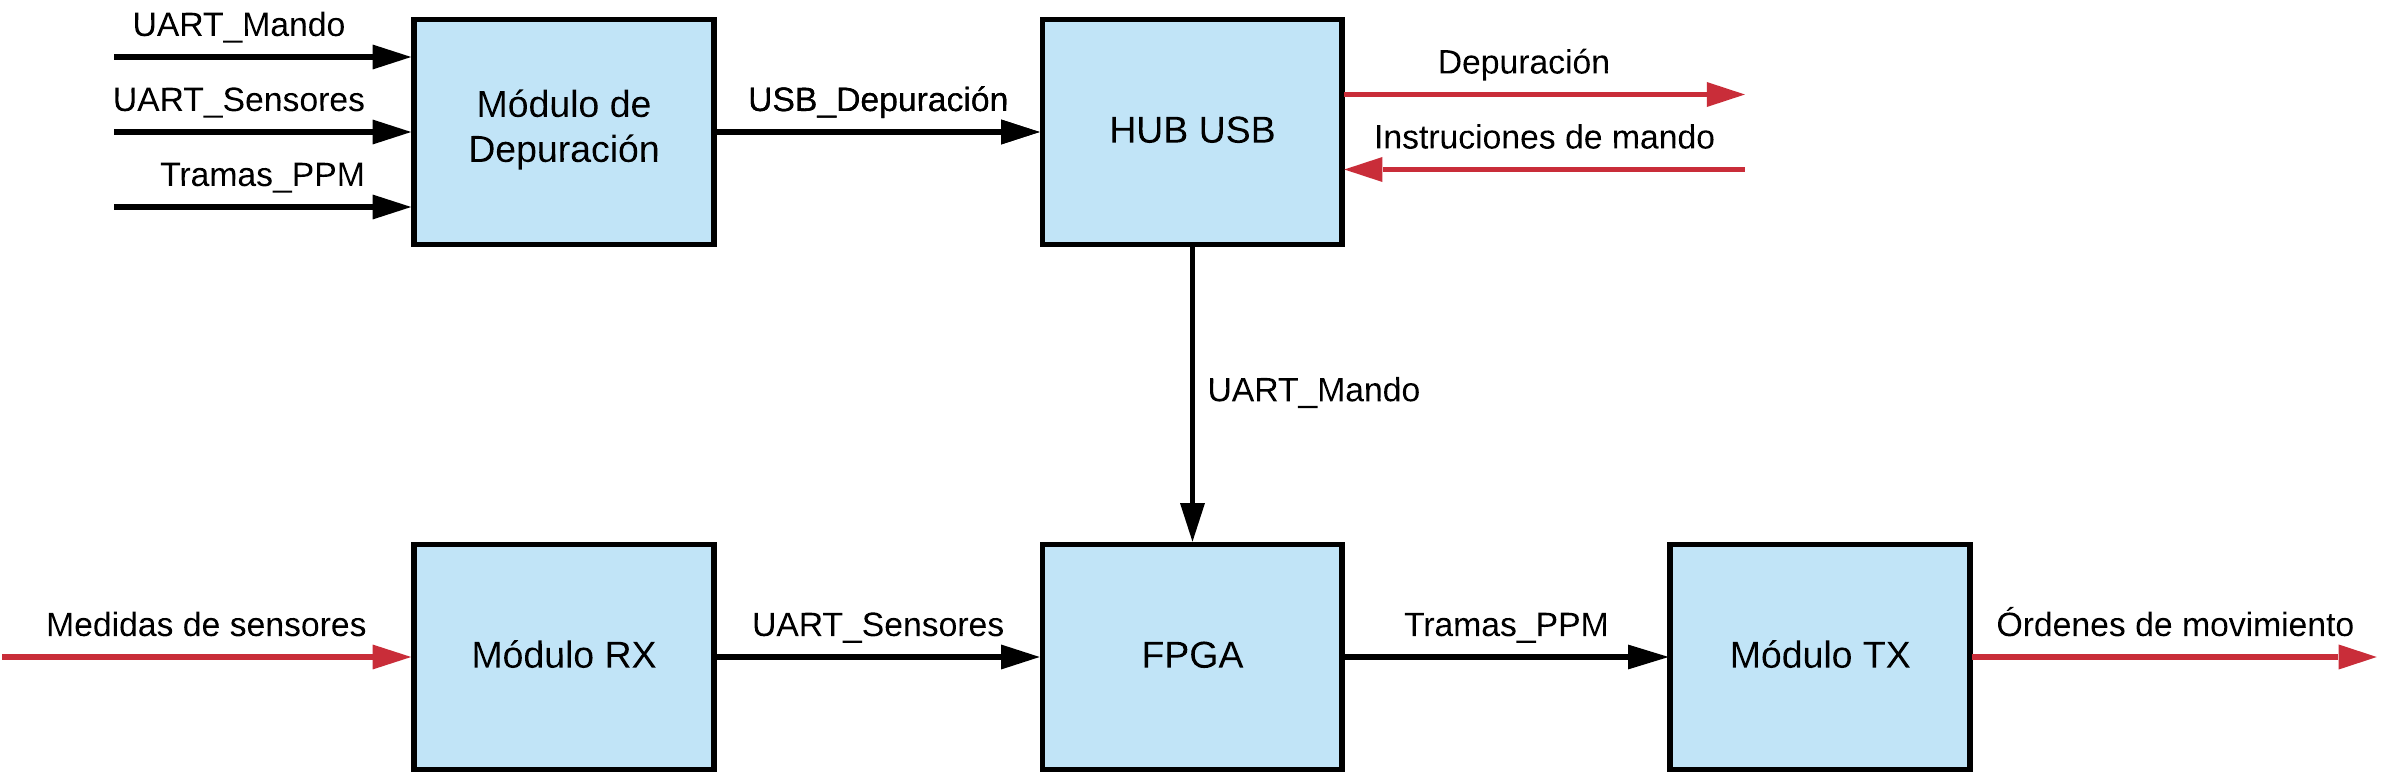
\includegraphics[width=11.5cm]{Imagenes/ET_arq}
		\end{figure}
	\end{center}
\end{minipage} \vfill
\begin{minipage}{20cm}
	\begin{minipage}{5.2cm}
		\begin{itemize}
			\item Atiende tramas de mando
			\item Atiende tramas desde dron
			\item Ejecuta algoritmos de control
		\end{itemize}
	\end{minipage}
	\begin{minipage}{6cm}
		\begin{itemize}
			\item Transmite \'ordenes de movimiento
			\item Encapsula depuraci\'on por USB
		\end{itemize}
	\end{minipage}
\end{minipage} \vfill
\end{hslide}
%%--------------------------------------------------------------
\begin{hslide}
\slsubsect{Estaci\'on de tierra basada en FPGA - Montaje}
\begin{minipage}{3cm}
	\begin{center}
		\begin{figure}
			\includegraphics[width=7.8cm]{Imagenes/Ground_Station_Mod}
		\end{figure}
	\end{center}
\end{minipage} \hfill
\begin{minipage}{2.8cm}
	M\'odulos:
	\begin{itemize}
		\item 1: Hub USB
		\item 2: FPGA
		\item 3: Receptor
		\item 4: Transmisor
		\item 5: Depuraci\'on
	\end{itemize}
\end{minipage}
\end{hslide}
%%--------------------------------------------------------------
\begin{hslide}
\slsubsect{Estaci\'on de tierra basada en FPGA - Algoritmo de control}
\begin{center}
	\begin{figure}
		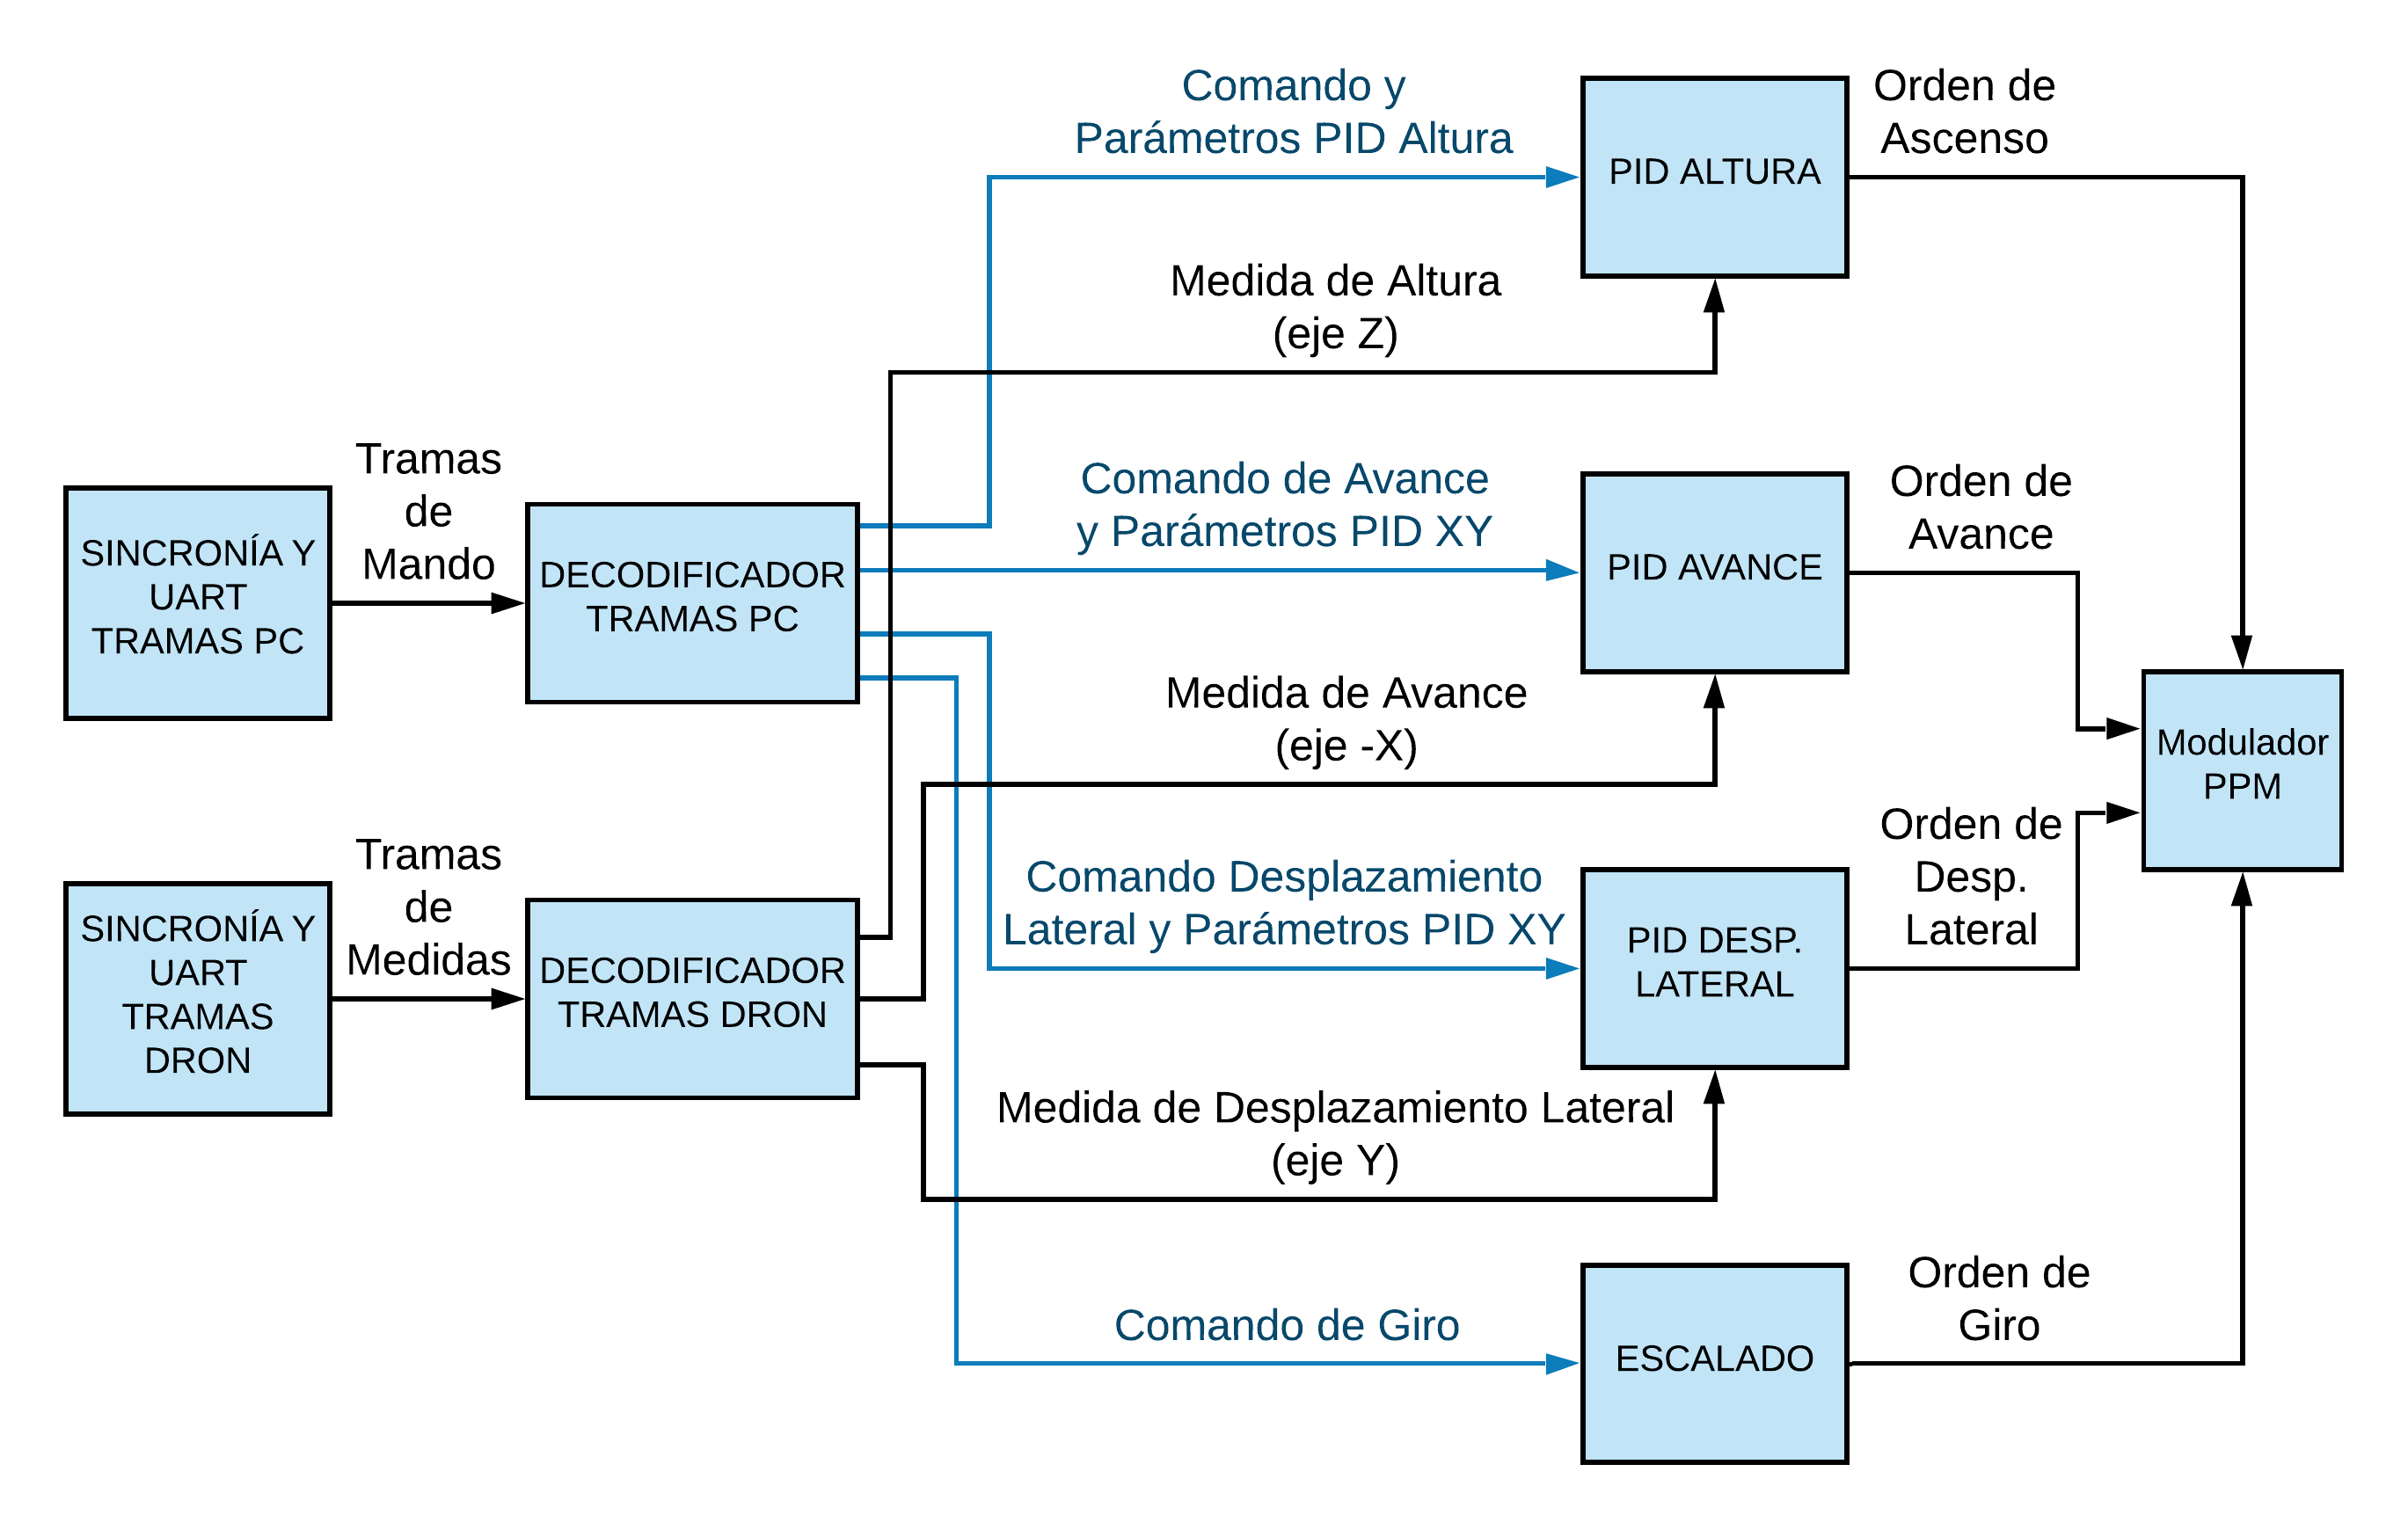
\includegraphics[width=12cm]{Imagenes/FPGA_New_Soft_arq}
	\end{figure}
\end{center}
\end{hslide}
%%--------------------------------------------------------------
\begin{hslide}
\slsubsect{Pc de Mando}
\begin{minipage}{2cm}
	\begin{center}
		\begin{figure}
			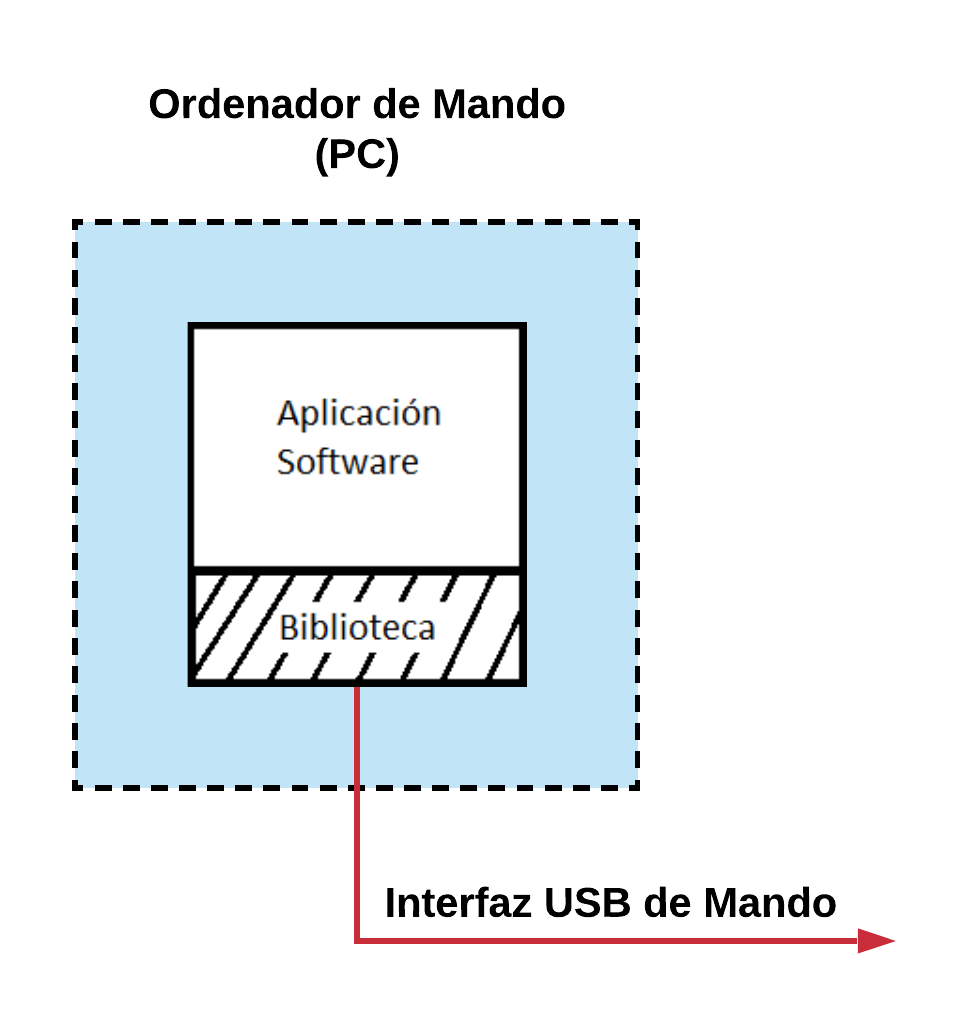
\includegraphics[width=5.5cm]{Imagenes/Arquitectura_del_Cod_PC}
		\end{figure}
	\end{center}
\end{minipage} \hfill
\begin{minipage}{6cm}
	\begin{itemize}
		\item Ejecuta instrucciones en Python
		\item Facilita el control del veh\'iculo
		\item Se comunica con la estaci\'on de tierra mediante USB
	\end{itemize}
\end{minipage}
\end{hslide}
%%--------------------------------------------------------------
\begin{hslide}
\slsubsect{Pc de Mando - Funciones}
\begin{center}


\begin{table}[H]
\resizebox{\textwidth}{!}{%
\begin{tabular}{|l|l|}
\hline
\texttt{setPIDValues} & Inicializaci\'on de valores de par\'ametros PID y ajuste de giro.                      \\ \hline
\texttt{setcontrols}  & Permite el control directo de los 4 grados de libertad disponibles en el veh\'iculo. \\ \hline
\texttt{settrace}     & Dirige una trayectoria progresiva entre la posici\'on actual y el punto indicado.    \\ \hline
\texttt{setcircle}     & Dirige una trayectoria progresiva en forma de arco entre la posici\'on actual y el \'angulo indicado.    \\ \hline
\texttt{takeoff}     & Arranca los motores y realiza el despegue hasta la altura indicada.    \\ \hline
\texttt{landing}     & Disminuye la altura progresivamente hasta el contacto con el suelo y apagado de motores.    \\ \hline
\end{tabular}
}
\end{table}



\end{center}
\end{hslide}



%%--------------------------------------------------------------
%% EXPERIMENTOS
%%--------------------------------------------------------------
\begin{hslide}
\slsect{Validaci\'on experimental}
\slsubsect{Dron \texttt{Eachine-E010}}
\begin{minipage}{20cm}
	\begin{minipage}{5.2cm}
		\begin{itemize}
			\item Ensayos de enlace radio
			\item Pruebas en bucle abierto
		\end{itemize}
	\end{minipage}
	\begin{minipage}{6cm}
		\begin{figure}
			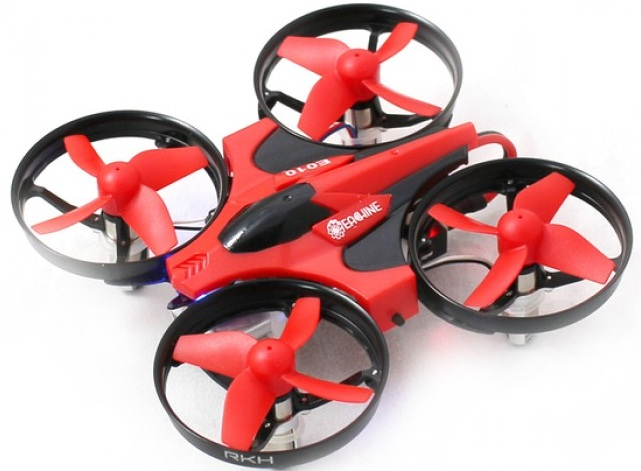
\includegraphics[width=1.8cm]{Imagenes/E010}
		\end{figure}
	\end{minipage}
\end{minipage} \vfill
\begin{minipage}{2cm}
	\begin{center}
		\begin{figure}
			\includegraphics[width=11.5cm]{Imagenes/Secuencia_7_flechas_amarillo}
		\end{figure}
	\end{center}
\end{minipage} \vfill
\end{hslide}
%%--------------------------------------------------------------
\begin{hslide}
\slsubsect{Dron \texttt{Syma-X5C}}
\begin{minipage}{20cm}
	\begin{minipage}{7.2cm}
		\begin{itemize}
			\item Modificaciones mayores
				\begin{itemize}
					\item Aligerado
					\item Sensorizaci\'on
					\item Transmisi\'on
				\end{itemize}
			\item Pruebas en bucle abierto y cerrado
		\end{itemize}
	\end{minipage}
\end{minipage} \hfill
\begin{minipage}{3cm}
	\begin{center}
		\begin{figure}
			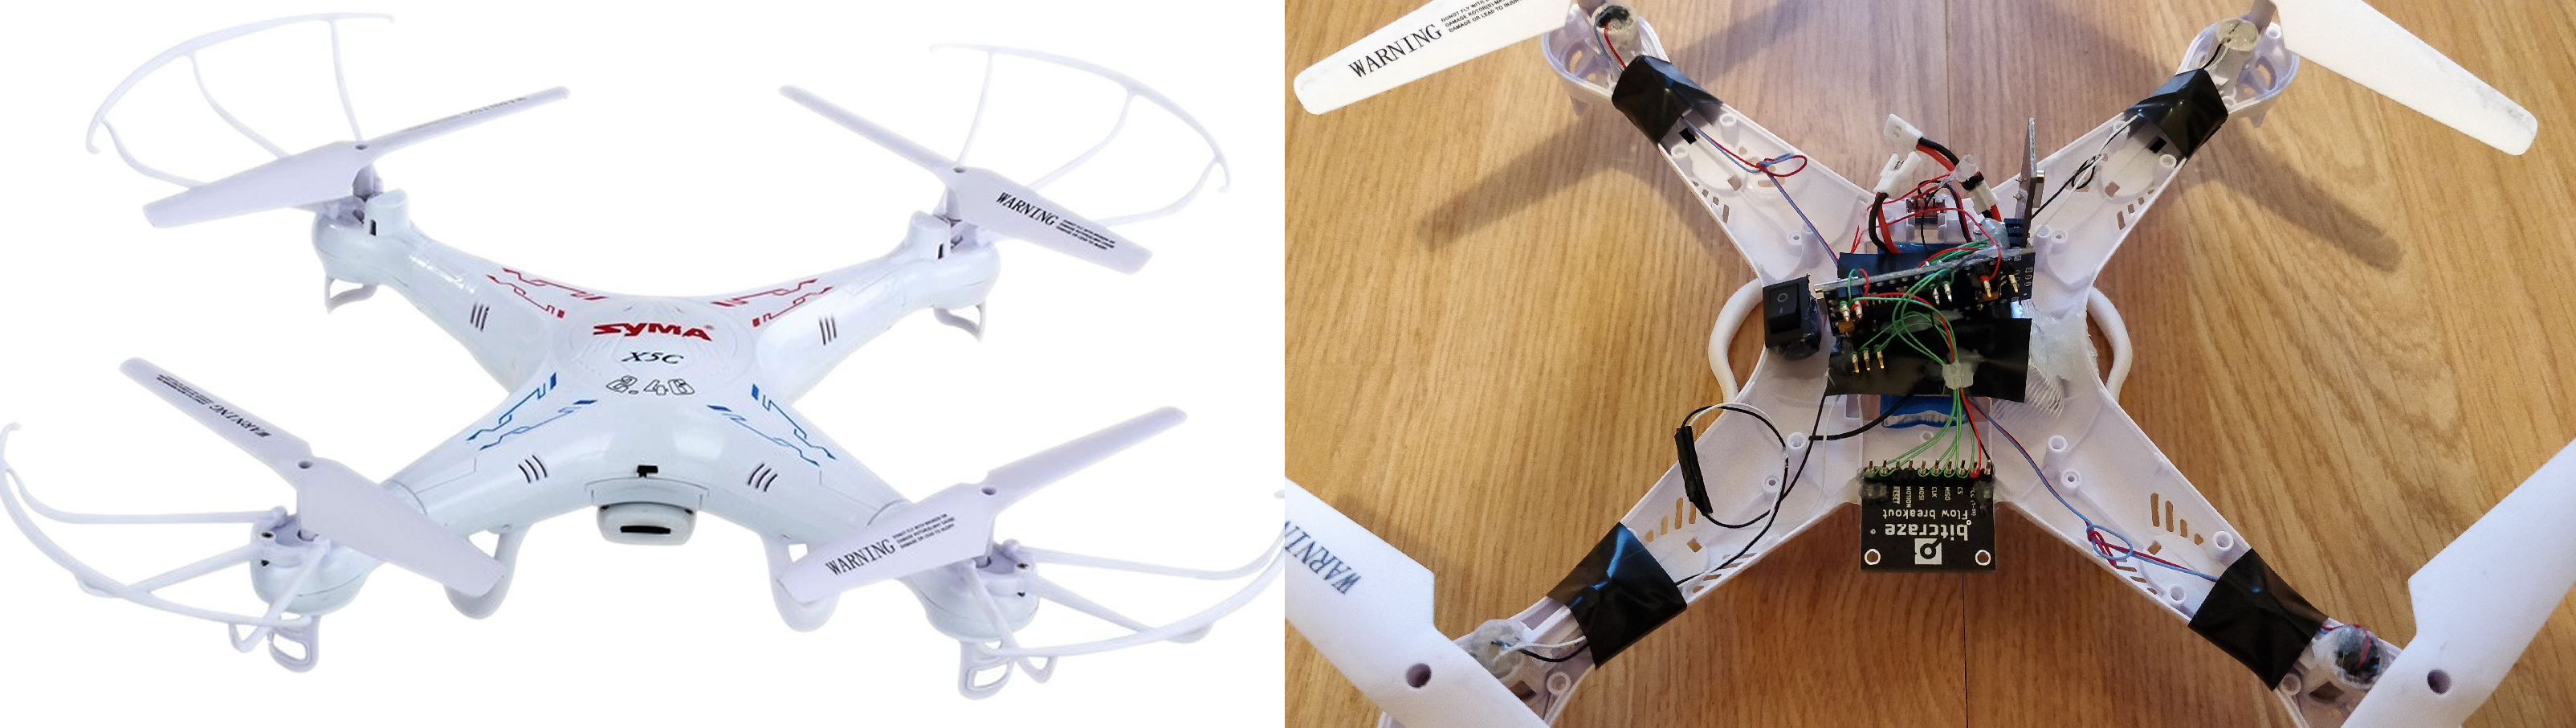
\includegraphics[width=11cm]{Imagenes/Syma_pre_post}
		\end{figure}
	\end{center}
\end{minipage} \vfill
\end{hslide}
%%--------------------------------------------------------------
\begin{hslide}
\slsubsect{Dron \texttt{Syma-X5C} Vuelo en Bucle Cerrado}
\begin{center}
	\begin{figure}
		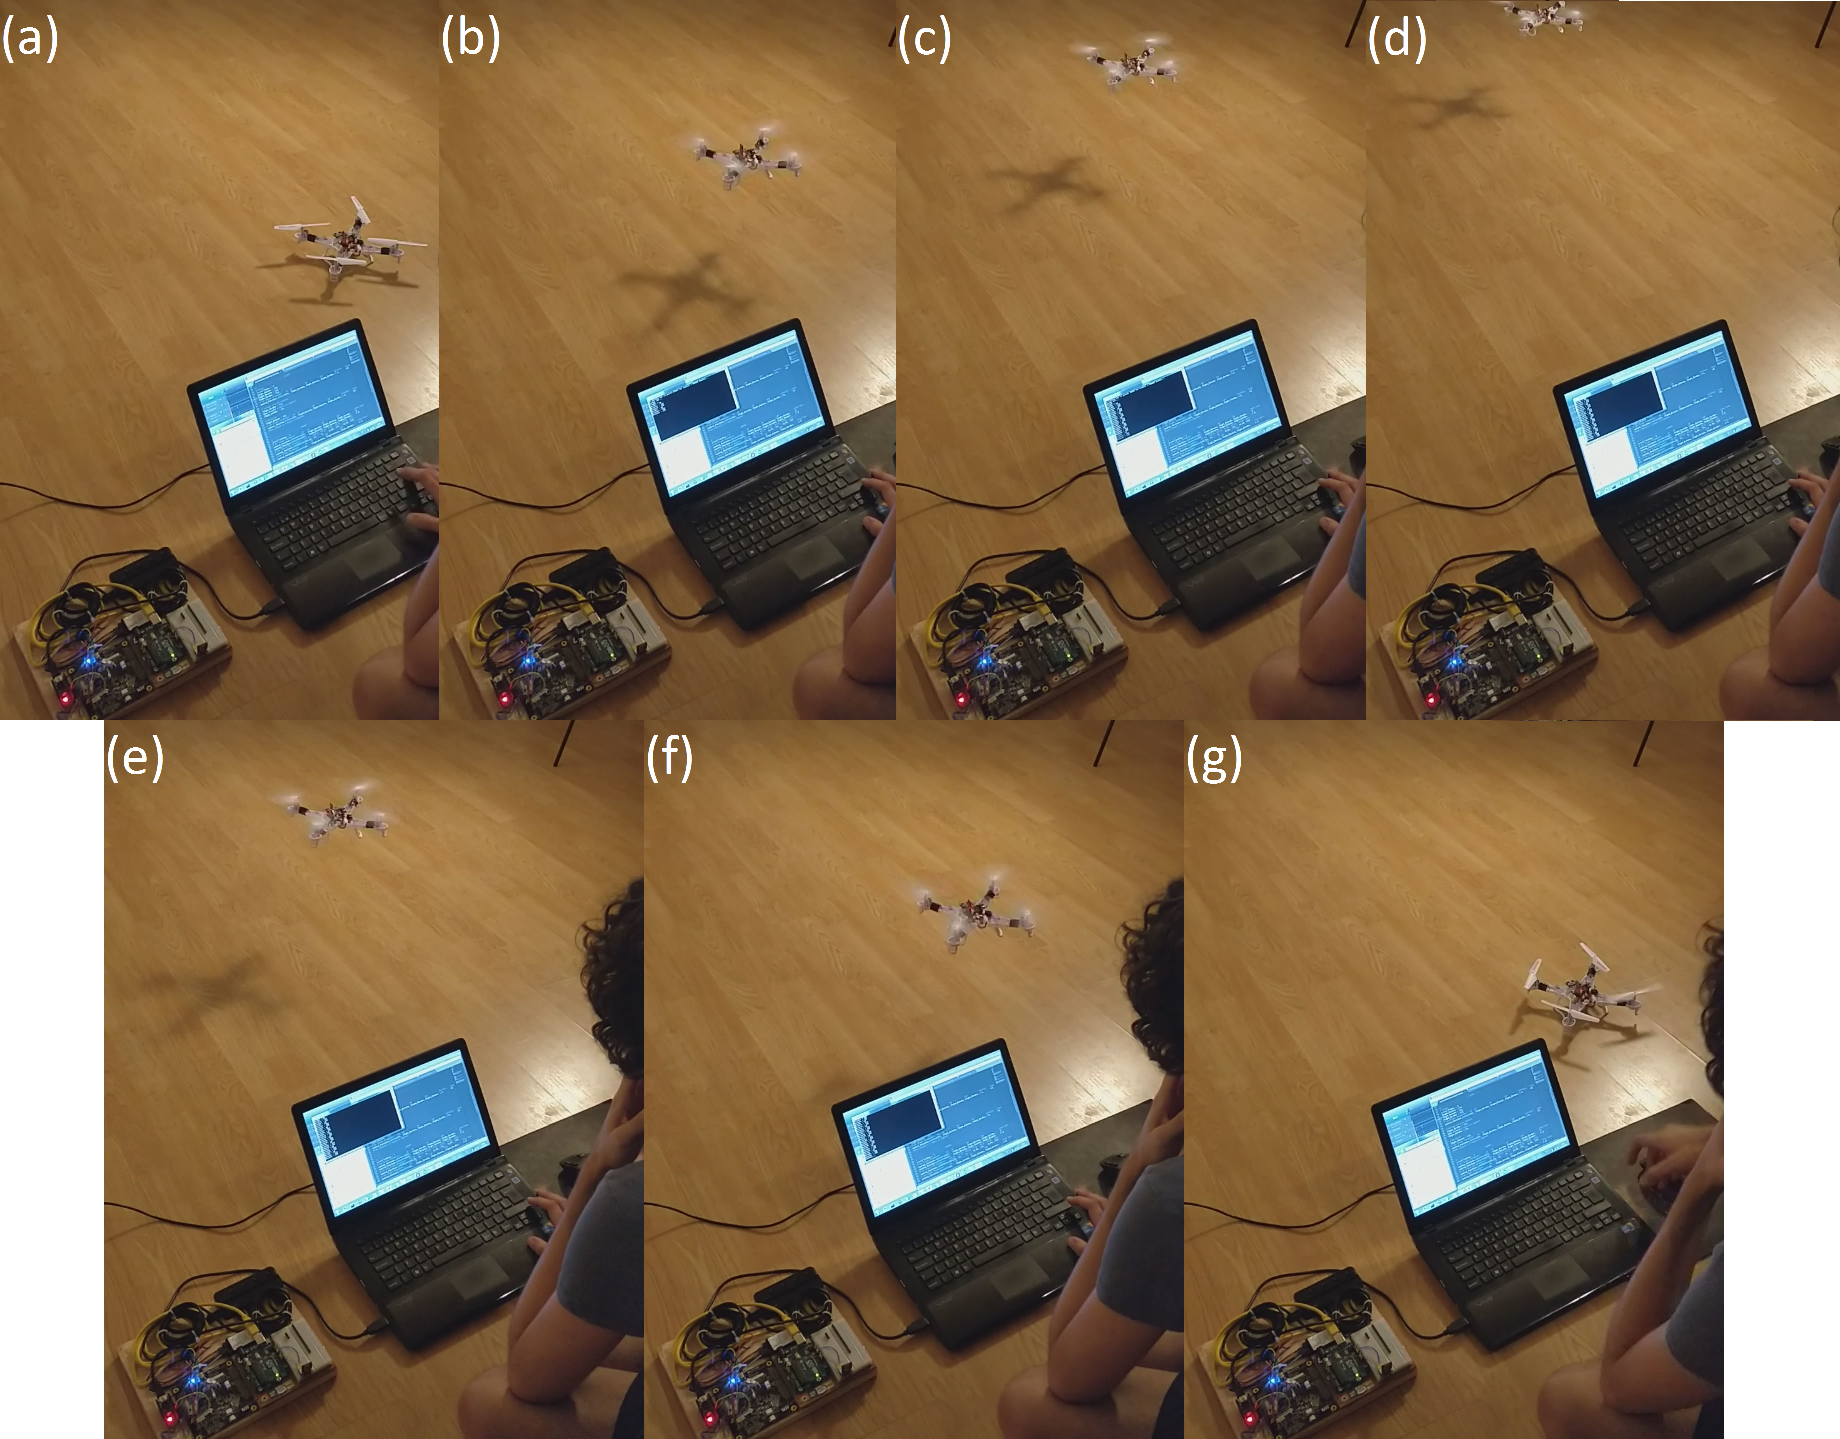
\includegraphics[width=9.1cm]{Imagenes/X5C_Secuencia_7_Small}
	\end{figure} \hfill
\end{center}
\end{hslide}



%%--------------------------------------------------------------
%% CONCLUSIONES
%%--------------------------------------------------------------
\begin{hslide}
\slsect{Conclusiones y l\'ineas futuras}
\begin{minipage}{8cm}
	\begin{itemize}
		\item Manejo b\'asico con bucles abiertos
		\item Resultado satisfactorio con bucles cerrados
			\begin{itemize}
				\item Estabilidad
				\item Control
				\item Repetitividad
			\end{itemize}
		\item Objetivos alcanzados con FPGAS y drones de muy bajo coste
		\item Ocupaci\'on de recursos de la FPGA al l\'imite de sus posibilidades
	\end{itemize}
\end{minipage} \hfill
\begin{minipage}{2cm}
	\begin{center}
		\begin{figure}
			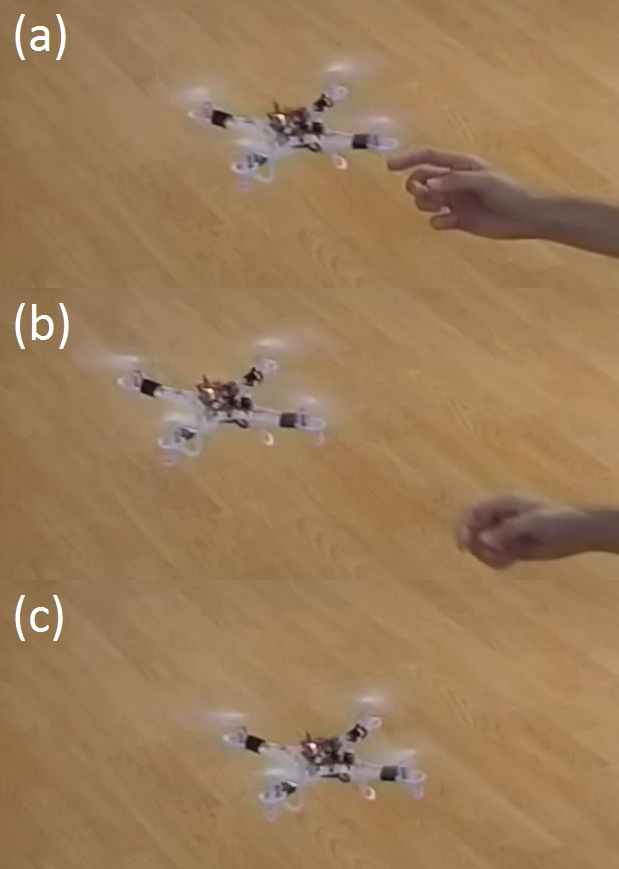
\includegraphics[width=3cm]{Imagenes/Interferencia_3_abc}
		\end{figure}
	\end{center}
\end{minipage} \hfill
\end{hslide}
%%---------------------------------------------------------------
\begin{hslide}
\slsubsect{L\'ineas futuras}

A\~nadidos de inter\'es
\begin{itemize}
	\item Magnet\'ometro para cierre de bucle de giro
	\item C\'amara y procesamiento de imagen
	\item GPS para ubicaci\'on global
\end{itemize}
Mejoras sobre el sistema actual
\begin{itemize}
	\item Mejoras software en eficiencia y disminuci\'on de latencias
	\item Bucles superiores de control: velocidad y aceleraci\'on
	\item Generador de trayectorias (ubicaci\'on conocida en PC de mando)
	\item Arquitectura basada en FPGA a bordo, con acceso a sensores y drivers
\end{itemize}


\end{hslide}
%%---------------------------------------------------------------

\end{document}\documentclass[notes,slidesec,a4]{seminar}


















%%--------------------------------------------------------------
%% Dron Syma-X5C validación experimetnal en una sola traspa
%%--------------------------------------------------------------
\begin{hslide}
\slsubsect{Dron \texttt{Syma-X5C}}
\begin{minipage}{5.5cm}
	\begin{minipage}{5cm}
		\begin{itemize}
			\item Modificaciones mayores
			\item Pruebas en bucle cerrado
		\end{itemize}
	\end{minipage}\vfill
	\begin{minipage}{6cm}
		\begin{figure}
			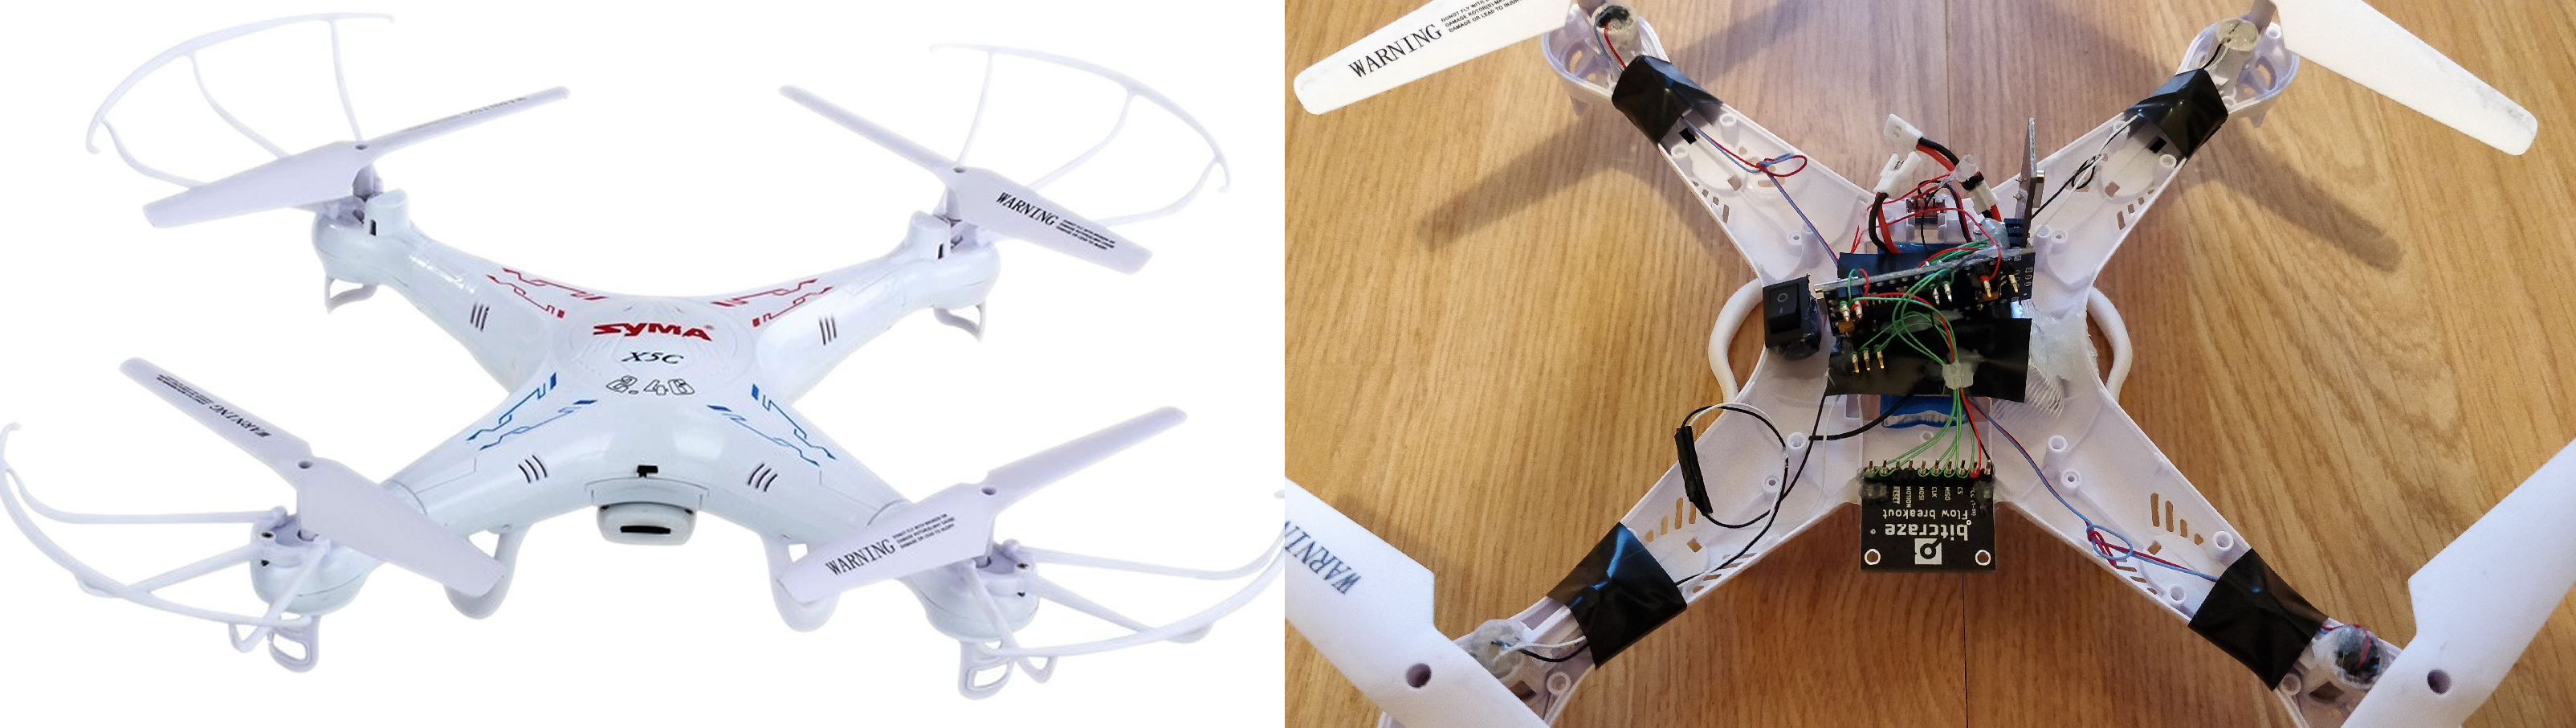
\includegraphics[width=5.5cm]{Imagenes/Syma_pre_post}
		\end{figure}
	\end{minipage}
\end{minipage}
\begin{minipage}{2cm}
	\begin{center}
		\begin{figure}
			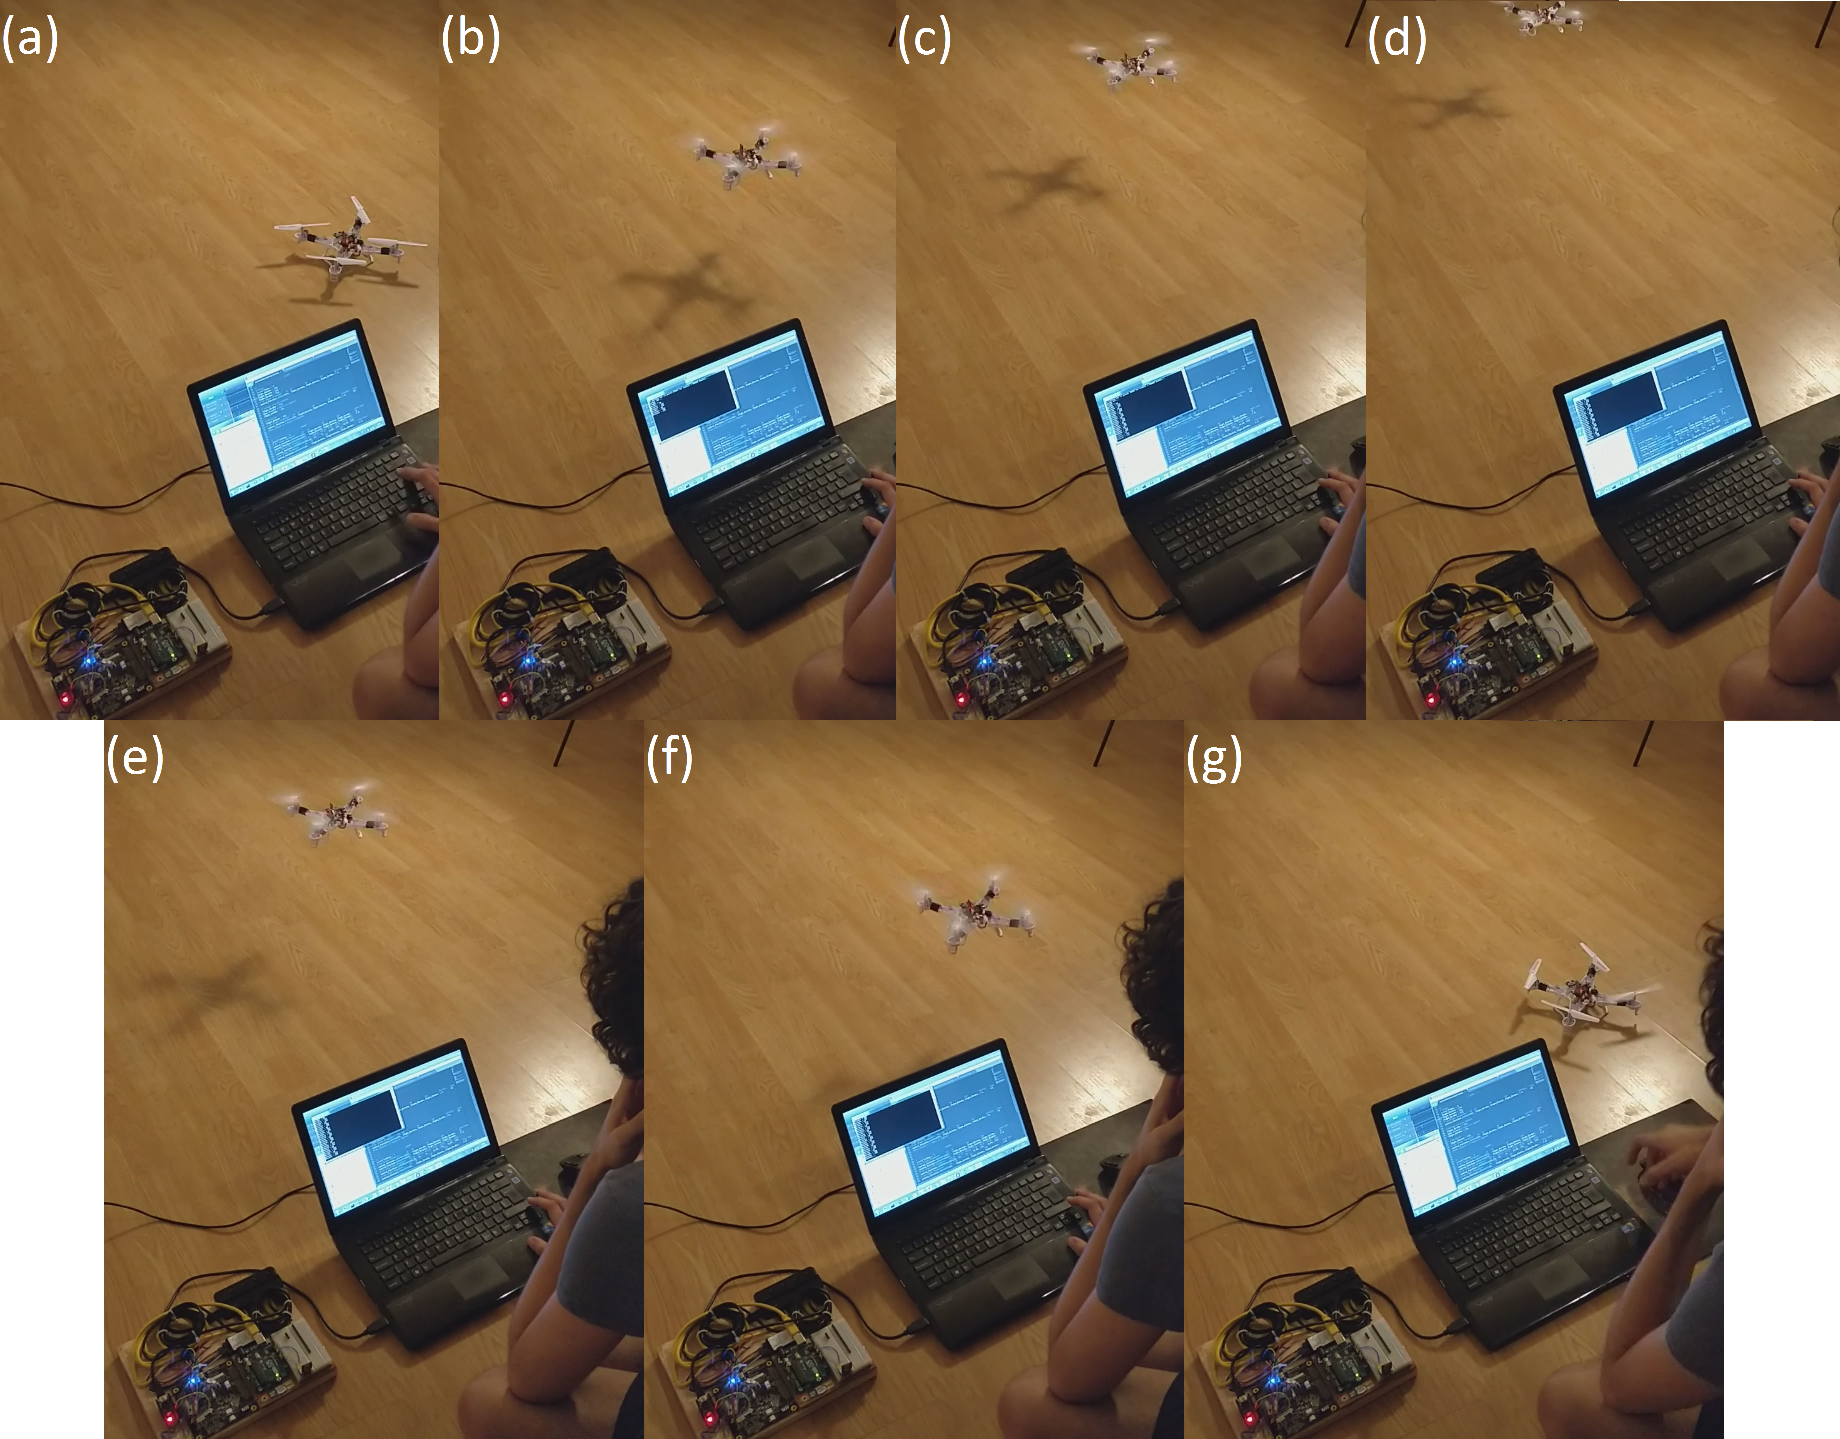
\includegraphics[width=7cm]{Imagenes/X5C_Secuencia_7_Small}
		\end{figure}
	\end{center}
\end{minipage} \hfill
\end{hslide}



%%---------------------------------------------------------------

\begin{hslide}
\slsubsect{}
\begin{minipage}{5cm}
	\begin{itemize}
		\item M\'as de una foto centrada en lado
	\end{itemize}
\end{minipage} \hfill
\begin{minipage}{2cm}
	\begin{center}
		\begin{figure}
			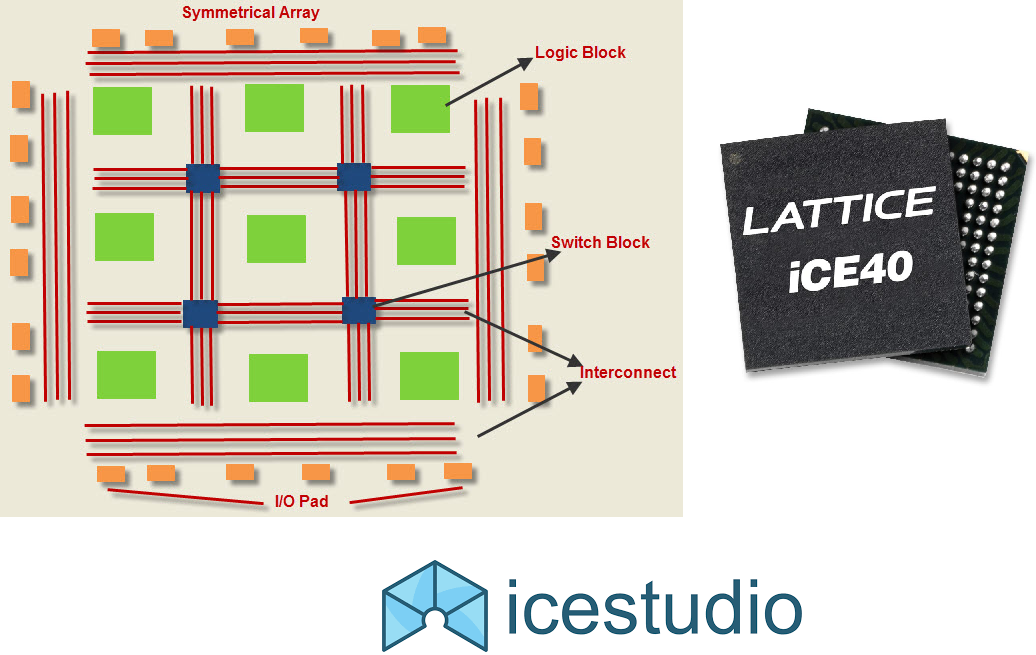
\includegraphics[width=2cm]{Imagenes/Intro_FPGA}
		\end{figure}
	\end{center}
\end{minipage} \hfill
\begin{minipage}{2cm}
	\begin{center}
		\begin{figure}
			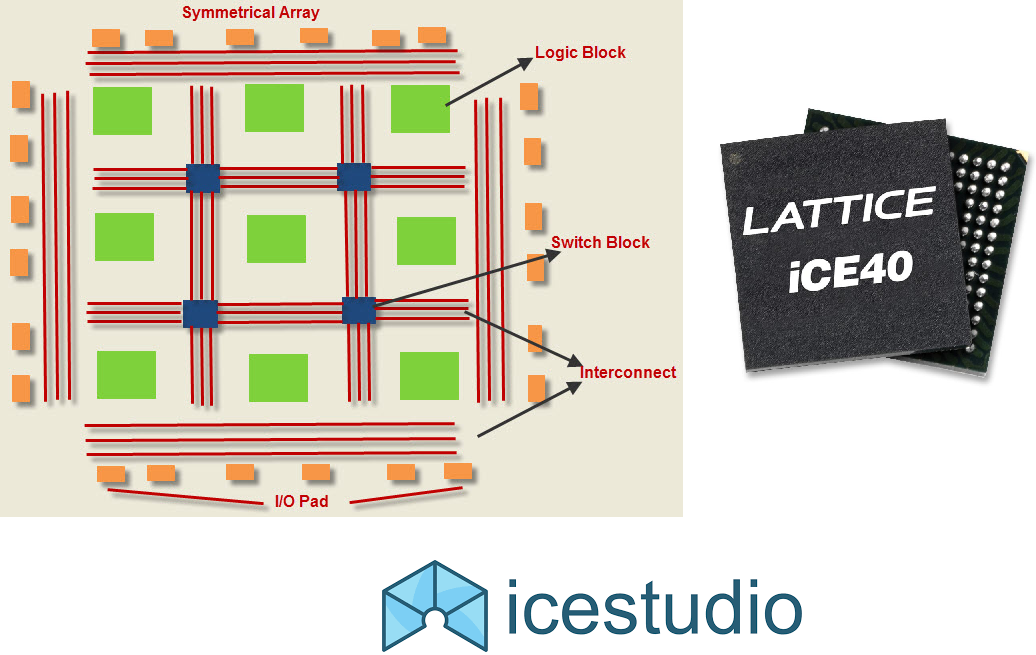
\includegraphics[width=2cm]{Imagenes/Intro_FPGA}
		\end{figure}
	\end{center}
\end{minipage}
\end{hslide}


%%---------------------------------------------------------------

\begin{hslide}
\slsubsect{Anidados}
\begin{minipage}{7cm}
	\begin{itemize}
		\item Nivel 1
		\begin{itemize}
			\item Nivel 2
		\end{itemize}
	\end{itemize}
\end{minipage} \hfill
\end{hslide}

%%---------------------------------------------------------------

\begin{hslide}
\slsubsect{Para c\'odigo - \texttt{aqu\'i}}

\end{hslide}